\documentclass[]{scrartcl}
\usepackage{lmodern}
\usepackage{amssymb,amsmath}
\usepackage{ifxetex,ifluatex}
\usepackage{fixltx2e} % provides \textsubscript
\ifnum 0\ifxetex 1\fi\ifluatex 1\fi=0 % if pdftex
  \usepackage[T1]{fontenc}
  \usepackage[utf8]{inputenc}
\else % if luatex or xelatex
  \ifxetex
    \usepackage{mathspec}
  \else
    \usepackage{fontspec}
  \fi
  \defaultfontfeatures{Ligatures=TeX,Scale=MatchLowercase}
\fi
% use upquote if available, for straight quotes in verbatim environments
\IfFileExists{upquote.sty}{\usepackage{upquote}}{}
% use microtype if available
\IfFileExists{microtype.sty}{%
\usepackage{microtype}
\UseMicrotypeSet[protrusion]{basicmath} % disable protrusion for tt fonts
}{}
\usepackage{hyperref}
\hypersetup{unicode=true,
            pdftitle={Angabe},
            pdfauthor={Team\ldots{}},
            pdfborder={0 0 0},
            breaklinks=true}
\urlstyle{same}  % don't use monospace font for urls
\IfFileExists{parskip.sty}{%
\usepackage{parskip}
}{% else
\setlength{\parindent}{0pt}
\setlength{\parskip}{6pt plus 2pt minus 1pt}
}
\setlength{\emergencystretch}{3em}  % prevent overfull lines
\providecommand{\tightlist}{%
  \setlength{\itemsep}{0pt}\setlength{\parskip}{0pt}}
\setcounter{secnumdepth}{5}
% Redefines (sub)paragraphs to behave more like sections
\ifx\paragraph\undefined\else
\let\oldparagraph\paragraph
\renewcommand{\paragraph}[1]{\oldparagraph{#1}\mbox{}}
\fi
\ifx\subparagraph\undefined\else
\let\oldsubparagraph\subparagraph
\renewcommand{\subparagraph}[1]{\oldsubparagraph{#1}\mbox{}}
\fi

\usepackage{graphicx}
\usepackage{array}
\usepackage{ragged2e}
\usepackage[section]{placeins}
\makeatletter
\AtBeginDocument{%
  \expandafter\renewcommand\expandafter\subsection\expandafter{%
    \expandafter\@fb@secFB\subsection
  }%
}
\makeatother

\title{Modell eines Insel-Callshops}
\providecommand{\subtitle}[1]{}
\subtitle{2. Projekt zu Modellierung und Simulation}
\author{Daniel Graf, Dimitrie Diez, Arne Schöntag, Peter Müller}
\date{}

\begin{document}

\maketitle

\tableofcontents
\section{Einführung}
Simulationen haben in der moderne einen sehr hohen Stellenwert erlangt, da durch sie zahlreiche, oftmals sehr genaue, Zukunftsprognosen erstellt werden können. Als Grundlage für die Simulationen dienen in der Regel Modelle, welche einen Ausschnitt der Wirklichkeit abbilden. Das Thema dieser Studienarbeit ist die Simulation eines Callshops, bzw. des Telefons in einem Callshop, in einem Inseldorf. Dieser wird für günstige Telefonate ins Ausland verwendet.

\section{Beschreibung des Modells}
Für die Simulation des Insel-Callshops wird ein Warteschlagenmodell mit Clients und zunächst nur einem Server verwendet. Jede Person die den CallShop betritt wird durch einen neuen Client repräsentiert. Das Telefon des Shops ist durch den Server dargestellt. Möchte eine Person das Telefon zu einem Zeitpunkt benützen, zu dem bereits eine andere Person telefoniert, muss sie sich hinten anstellen und warten, bis die Person ihr Telefonat beendet hat. Im Modell wird dieses durch eine Warteschlage (Queue) realisiert, in die sich ankommende Clients einordnen und sobald der Server nichtmehr belegt ist nach dem FIFO (first in first out) Prinzip bedient werden.

Im Modell werden sowohl die Ankunftszeiten der Clients, als auch die Dauer der Telefonate durch eine negative Exponentialverteilung beschrieben, da diese sehr nah an den real beoachteten Verhalten liegt. Der mathematische Hintergrund liegt in der Eigenschaft der Exponentialfunktion zugrunde. Die Exponentialverteilung ist die einzige kontinuierliche Verteilung, welche zugleich die Markoveigenschaft, die sogenannte Gedächtnislosigkeit, erfüllt. Diese besagt, dass die seit dem letzten Ereignis vergangene Zeit (in diesem Beispiel Anrufer) keinen Einfluss auf die Verteilung der Zeit bis zum nächsten Ereignis (bis zum nächsten Anruf) hat \cite{ExpoVert}.

Darüber hinaus wird ein zweites Modell betrachtet, in welchem die Bewohner des Inseldorfes (Einheimische) bevorzugt werden. Im weiteren Verlauf der Studienarbeit werden diese als VIP oder resident bezeichnet. Der grundlegende Ablauf verläuft wie beim ersten Modell. Allerdings wird, bevor der nächste Client (FIFO Prinzip) telefonieren darf, die Queue nach einem Einheimischen durchsucht. Befindet sich ein Einheimischer in der Queue, wird dieser bevorzugt und darf zuerst telfonieren. Alle restlichen Kunden in der Queue (im folgenden als Touristen bezeichnet) müssen warten bis sich kein Einheimischer mehr in der Warteschlange befindet.

In einem dritten Modell befindet sich ein weiteres Telefon im Callshop. Von den nun zwei Telefonen (zwei Server), behandelt eines alle ankommenden Personen (Clients) gleichberechtigt (analog zum ersten Modell). Das zweite Telefon bevorzugt die Einheimischer und behandelt Touristen nur, wenn kein Einheimischer wartet (analog zum zweiten Modell).

\section{Anforderungen/Requirements}
\label{requirements}
\subsection{Allgemeines}
Die Software soll die Simulation eines Warteschlangensystems durchführen. Zu Beginn der Simulation wird davon ausgegangen, dass die Warteschlange keine Elemente enthält, da sich auch in der Realität beim Öffnen eines Ladens noch keine Personen in einer Warteschlange im Laden befinden.
\subsection{Verteilung der Zwischenankunfszeiten}
Die Zwischenankunftszeiten sollen zufällig genieriert werden. Die Verteilung der Zufallszahlen soll eine negative Exponentialverteilung aufweisen. Die Exponentialverteilung für eine zufällige Zwischenankunftszeit x ist erfüllt falls sie folgende Dichtefunktion besitzt:
$$
f(x) = \left\{\begin{matrix}
\lambda e^{-\lambda x}
\\
0
\end{matrix}\right.für \begin{matrix}
x \geqslant 0
\\
x < 0
\end{matrix}
$$
Die mittlere Zwischenankunftszeit hat den Erwartungswert $\frac{1}{\lambda}$. Die mittlere Zwischenankunftszeit soll parametrisierbar sein.
\subsection{Verteilung der Telefonierzeiten}
Die Telefonierzeiten sollen zufällig generiert werden. Die Verteilung der Zufallszahlen soll analog zur Zwischenankunftszeiten eine Exponentialverteilung aufweisen. Die mittlere Telefonierzeit soll ebennfalls parametrisierbar sein.

\subsection{Zeitmodelierung}
Die Applikation unterliegt keinen harten Echtzeitanforderungen. Die Simulation soll für die gesamte Simmulationsdauer so schnell wie möglich durchgeführt werden. Es soll keine Globale Uhr modelliert werden.

\subsection{Berechnungen}
Die Funktion der Applikation ist die Simulation eines Warteschlangenmodells und die Berechnung relevanter Daten. Alle Werte werden mit Hilfe der Java Klasse BigDecimal berechnet. Für die Division werden 32 Nachkommastellen berücksichtigt und als Rundungsmodus wird Half\_Even verwendet, da dieser kumulative Fehler bei sich wiederholenden Berechnungen minimiert.
Die Auswertung und grafische Darstellung der Daten erfolgt mit Mathematica.

\subsection{Reports}
Alle errechneten Ergebnisse sollen über Reports ausgeleitet werden. Die Reports sollen im .csv Format ausgeleitet werden um eine gute Weiterverarbeitung der Ergebnisse zu gewährleisten. Folgende Reports sollen ausgeleitet werden:
\begin{list}{•}
	\item arrival-delta.csv enthält alle Zwischenankunftszeiten einer Simulation

	\item serve-delta.csv enthält alle Telefonierzeiten

	\item little-system-all.csv enthält alle Werte für die Gleichung \ref{eq:little}

    	\item little-system-normal.csv enthält die Werte der Touristen für die Gleichung \ref{eq:little}

    	\item little-system-resident.csv enthält die Werte der Einheimischen für die Gleichung \ref{eq:little}
    	\item mean-phone-size-all.csv enthält die durchschnittliche Auslastung des Telefons
    	\item mean-queue-size-all.csv enthält die durchschnittliche Warteschlangenlänge
    	\item mean-queue-size-normal.csv enthält die durschnittliche Warteschlangenlänge der Touristen
    	\item mean-queue-size-resident.csv enthält die durchschnittliche Warteschlangenlänge der Einheimischen
    	\item mean-system-size-all.csv enthält die durchschnittliche Anzahl an Kunden im System
    	\item mean-system-size-normal.csv enthält die durschnittliche Anzahl an Touristen im System
    	\item mean-system-size-resident.csv enthält die durchschnittliche Anzahl an Einheimischen im System
    	\item mean-queue-time-all.csv enthält die durchschnittliche Wartezeit aller Kunden
    	\item mean-queue-time-normal.csv enthält die durschnittliche Wartezeit der Touristen
    	\item mean-queue-time-resident.csv enthält die durchschnittliche Wartezeit der Einheimischen
    	\item mean-system-time-all.csv enthält die durchschnittliche Verweildauer der Kunden im System
    	\item mean-system-time-normal.csv enthält die durschnittliche Verweildauer der Touristen im System
    	\item mean-system-time-resident.csv enthält die durchschnittliche Verweildauer der Einheimischen im System
    	\item queue-size-all.csv enthält die Länge der gesamten Warteschlange zu den jeweiligen Zeitpunkten
    	\item queue-size-tourist.csv enthält die Länge der Touristen-Warteschlange zu den jeweiligen Zeitpunkten
    	\item queue-size-resident.csv enthält die Länge der Einheimischen-Warteschlange zu den jeweiligen Zeitpunkten

\end{list}
\subsection{Parameter}
Die Tabelle \ref{tab:parameter} zeigt alle möglichen Parameter, welche die Software steuern. Alle Parameter sind optional.
\begin{table}[htpb]
	\centering
	\begin{tabular}{lll}
		Parameter & Beschreibung  &  Default\\ \hline
		-a & durschnittliche Zwischenankunftszeit der Besucher in Sekunden [s] & 1000 \\
		-c & durschnittliche Telefonierdauer in Sekunden [s] & 100 \\
		-d & Dauer der Simulation in Sekunden [s] & 100.000.000 \\
		-vip & Anteil der Inselbewohner an den Besuchern in Prozent [\%] &  10 \\
		-conf & Betriebsmodus (1, 2, oder 3) & 1 \\
		-o & Ausgabepfad zur Reporterstellung & ../data/
	\end{tabular}
	\caption{Parameter und Defaultwerte}
	\label{tab:parameter}
\end{table}


\subsection{Betriebsmodi}
Die Software hat drei Betriebsmodi:
\begin{list}{}
	\item Betriebsmodus 1: In diesem Modus gibt es ein Telefon und eine Warteschlange. Alle Personen in der Warteschlange werden gleichberechtigt behandelt.
	\item Betriebsmodus 2: In diesem Modus gibt es ein Telefon und eine Warteschlange. Die Personen werden jedoch unterschieden nach Einheimischen (VIP) und Touristen. Einheimische werden bevorzugt behandelt. Befindet sich ein Einheimischer in der Warteschlange, wird dieser zuerst telefonieren, sobald das Telefon frei ist. Befinden sich mehrere Einheimische in der Warteschlange, wird der erste zuerst abgearbeitet. Das Verhältnis von Einheimischen zu Touristen kann mittels des Parameters percVIP geregelt werden.
	\item Betriebsmodus 3: In diesem Modus gibt es eine Warteschlange und zwei Telefone. Das erste Telefon behandelt die Warteschlange analog zu Betriebsmodus 2. Das zweite Telefon behandelt die Warteschlange der Reihe nach unabhängig davon, ob es sich um einen Touristen oder einen Einheimischen handelt.
\end{list}

\subsection{Werte für die Auswertung}
Alle in der Tabelle \ref{tab:WerteAuswertung} aufgeführten Werte sollen auf Basis der Simulation ermittelt und ausgewertet werden.
\begin{table}[htpb]
	\centering
	\begin{tabular}{lll}
		Ermittelte Werte & Beschreibung \\ \hline
		Mittlere Warteschlangenlänge & Durchschnittliche Anzahl der anstehenden Kunden \\
		Mittlere Anstehzeit & Durchschnittliche Wartezeit eines Kunden \\
		Mittlere Verweildauer im Shop & Mittlere Anstehzeit + Mittlere Telefonierdauer\\
		Mittlere Serverauslastung & Anteil an der Gesamtzeit, in der das Telefon belegt ist\\
	\end{tabular}
	\caption{Werte für die Auswertung}
	\label{tab:WerteAuswertung}
\end{table}


\section{Softwaredesign}

Der Aufbau der Anwendung wurde im Team diskutiert und anschließend mittels UML spezifiziert.

Grundsätzlich wurde eine Ereignisorientierte Simulation (Discrete Event Simulation) mit einer Eventliste gewählt. Ursprünglich war geplant die Berechnung mit Mathematica auszuführen. Dies stellte sich aber als nicht performant und komplizierter als notwendig heraus. Alle geforderten Berechnungen wurden dann ebenfalls in das Java Programm eingeplant.

\subsection{Package time}

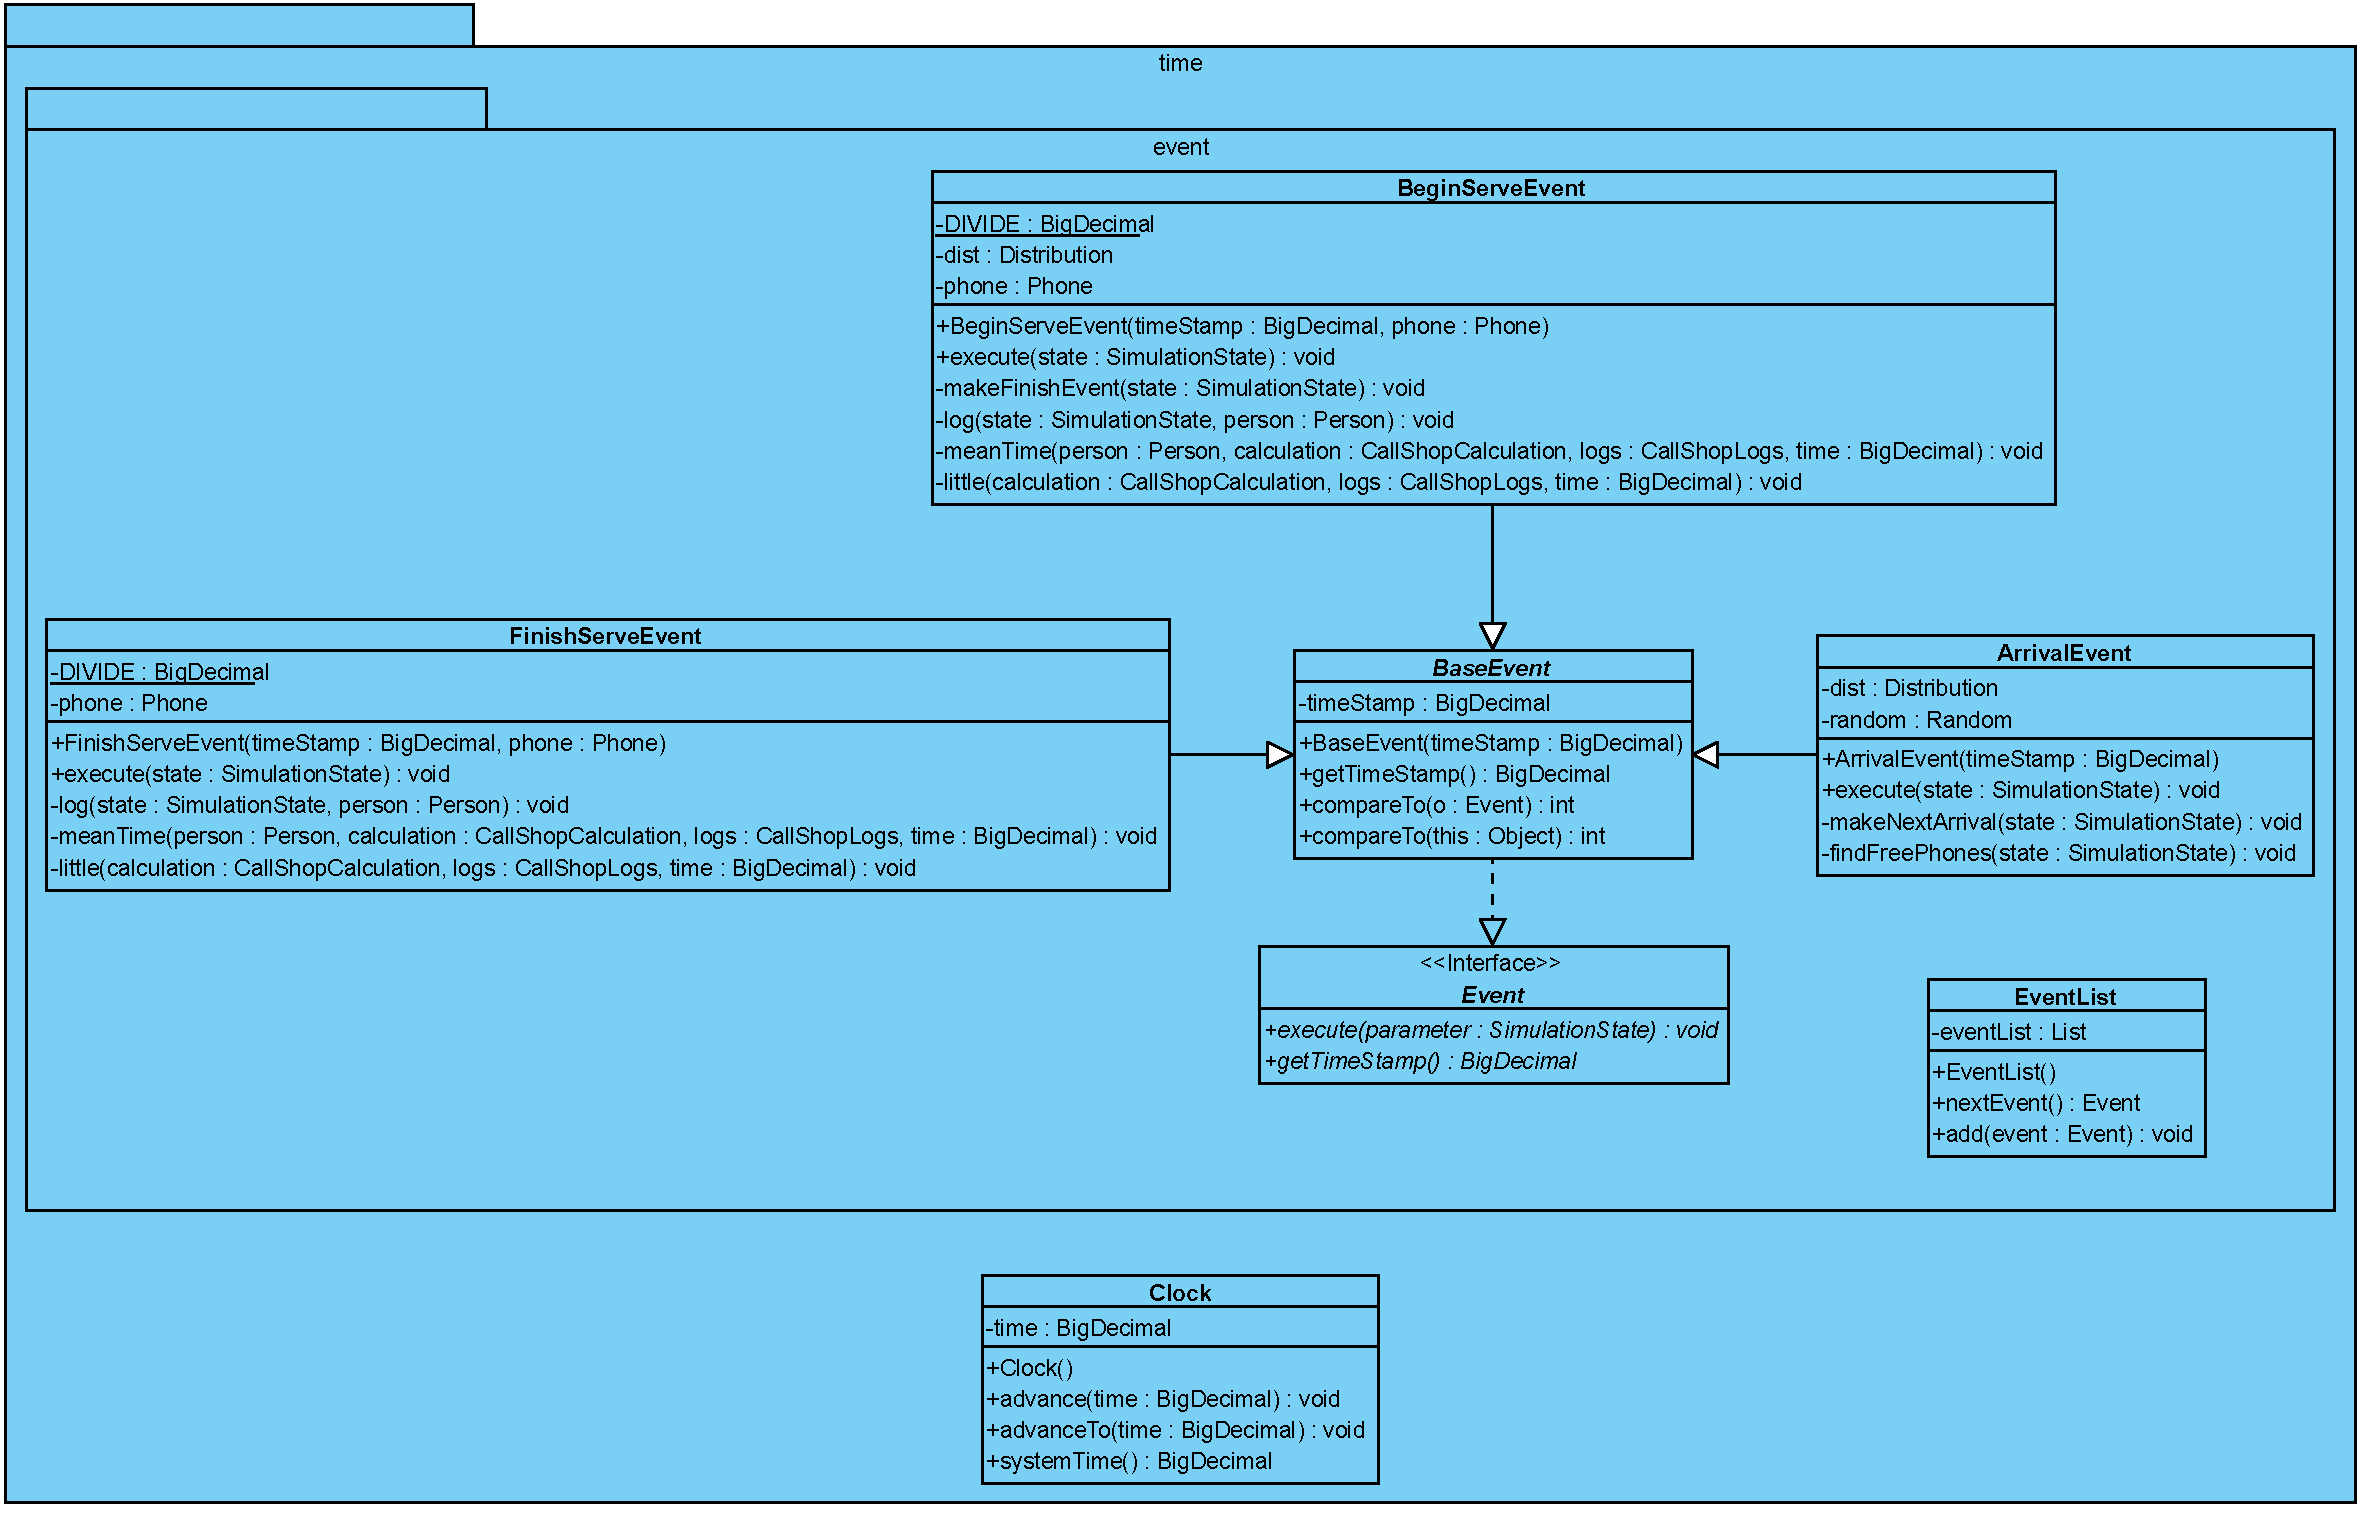
\includegraphics[scale=0.5]{abbildungen/uml/time.pdf}

In diesem Unterpaket finden sich alle notwendigen Klassen für die Ereignisorientierte Simulation. Die \texttt{Clock} hält die Simulationszeit und kann nur vorgestellt werden.

Das Interface \texttt{Event} definiert ein Ereignis in der Simulation. Jedes Ereignis hat einen Zeitpunkt an dem es auftritt, sowie Logik, die zu diesem Zeitpunkt ausgeführt werden soll und potentiell den ganzen Zustand der Simulation verändern kann. Die \texttt{EventList} kann Ereignisse aufnehmen und immer das nächste Event mit den frühesten Zeitpunkt liefern.

Die konkreten Events \texttt{Arrival, BeginServe, FinishServe} beschreiben die Ereignisse in der Callshop Problemstellung.

Abbildung \ref{fig:arrival-event} zeigt den Verlauf des Ereignisses für Arrival. Zunächst werden freie Telefone gesucht. Wird ein freies Telefon gefunden wird ein BeginServeEvent mit aktueller Zeit erstellt. Eine neue Person wird erstellt, ihre Ankunftszeit gespeichert, und die Person wird in die Schlange eingefügt. Zum Schluss wird das nächste ArrivalEvent erstellt, um fortlaufend neue Ankünfte zu haben.

Der Verlauf von BeginServe ist in Abbildung \ref{fig:beginserve-event} zu sehen. Die nächste (VIP oder normale) Person wird je nachdem, ob es sich um ein VIP Phone oder nicht handelt, aus der Liste geholt. Die Zeit vom Bearbeitungsbeginn wird für die Person gespeichert. Das FinishEvent wird direkt ermittelt und in die EventList eingetragen.

Das Ereignis FinishServe ist in Abbildung \ref{fig:finishserve-event} dargestellt. Die Person wird aus dem Phone entfernt. Ihre Endzeit wird gespeichert. Ist die Warteschlange nicht leer, wird direkt ein neues BeginServeEvent erstellt.


\begin{figure}[ht]
	\centering
	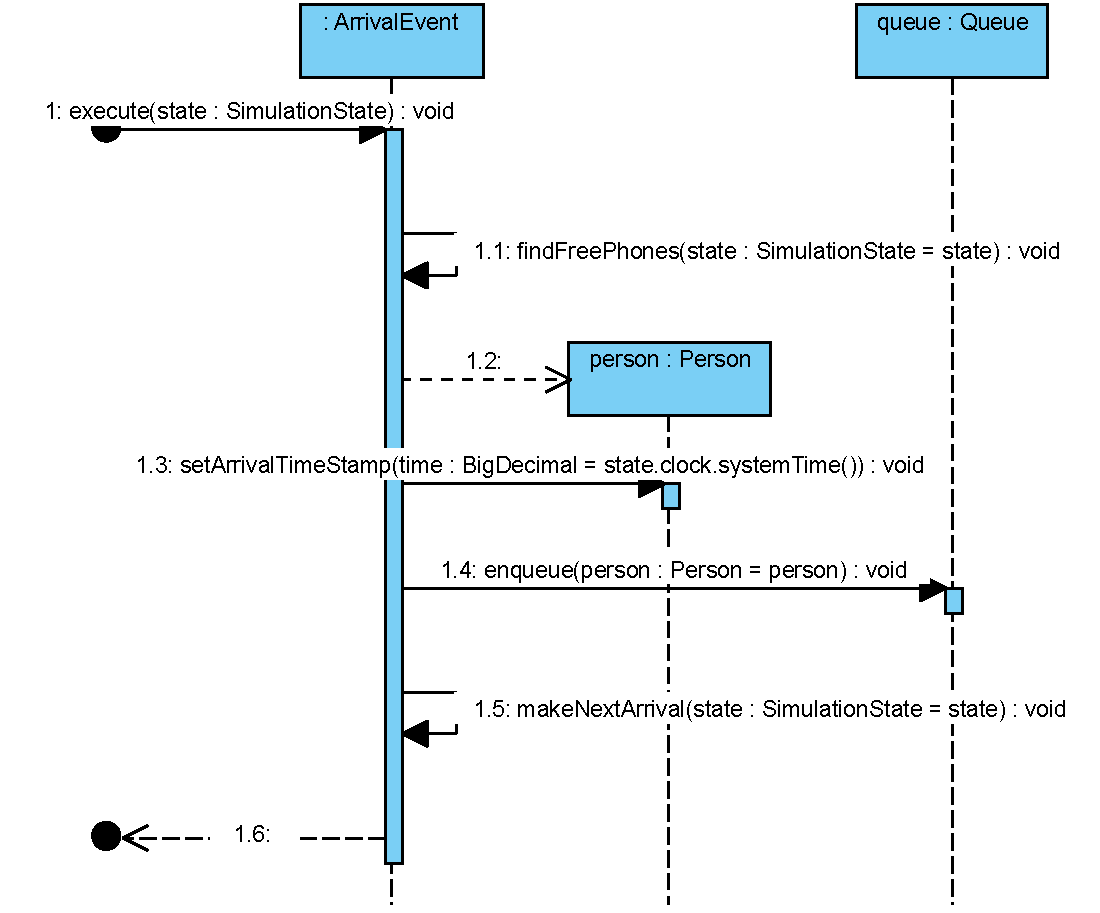
\includegraphics[scale=0.5]{abbildungen/uml/Arrival.pdf}
	\caption{Sequenzdiagramm für die Ausführung eines ArrivalEvent}
	\label{fig:arrival-event}
\end{figure}

\begin{figure}[ht]
	\centering
	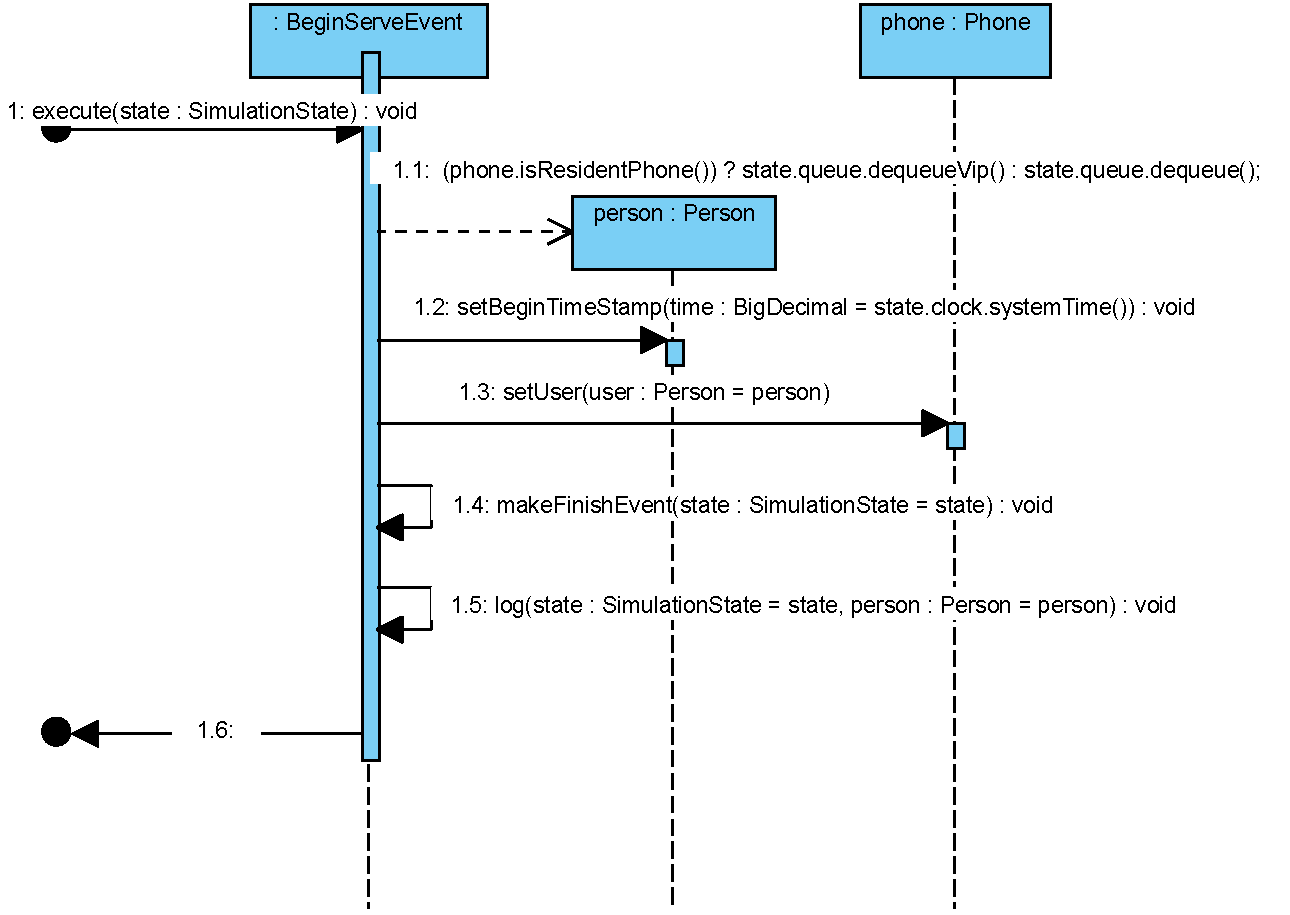
\includegraphics[scale=0.5]{abbildungen/uml/BeginServe.pdf}
	\caption{Sequenzdiagramm für die Ausführung eines BeginServeEvent}
	\label{fig:beginserve-event}
\end{figure}

\begin{figure}[ht]
	\centering
	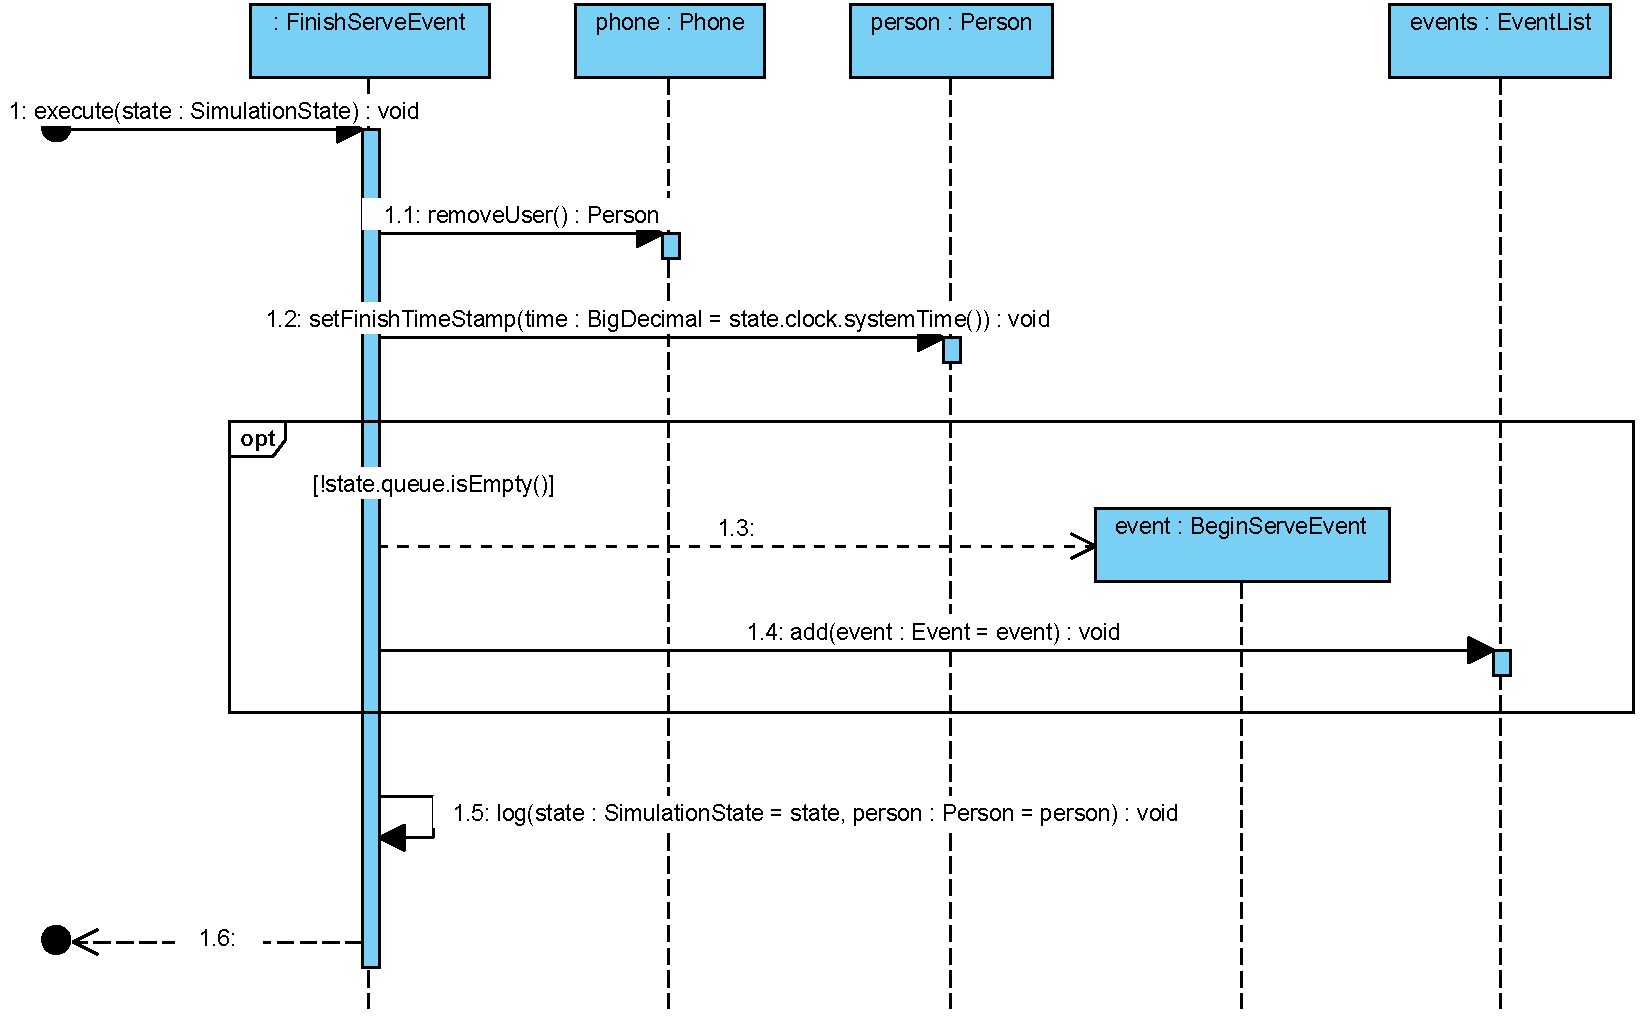
\includegraphics[scale=0.5]{abbildungen/uml/FinishServe.pdf}
	\caption{Sequenzdiagramm für die Ausführung eines FinishServeEvent}
	\label{fig:finishserve-event}
\end{figure}

\subsection{Package queue}

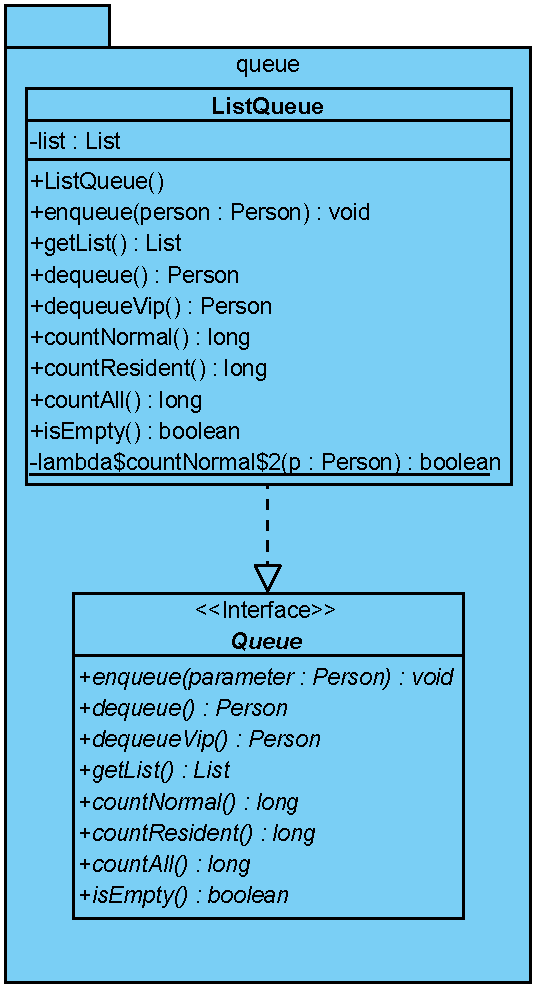
\includegraphics[scale=0.5]{abbildungen/uml/queue.pdf}

Die \texttt{Queue} ist eine FIFO-Warteschlange mit zugehörigen Operationen. Optional kann direkt auch der erste Resident (VIP) aus der Schlange entfernt werden.

\subsection{Package distribution}

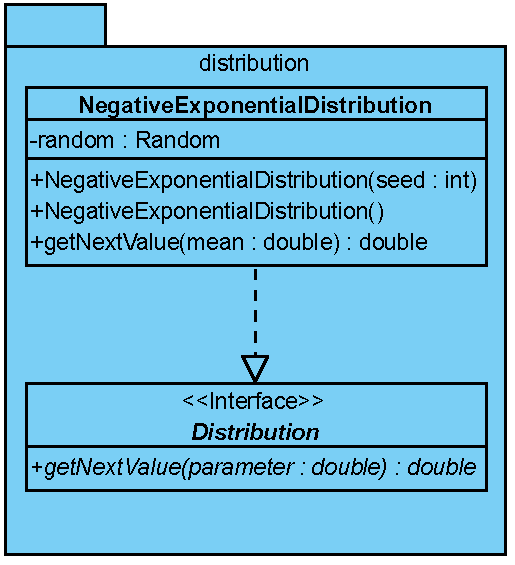
\includegraphics[scale=0.5]{abbildungen/uml/distribution.pdf}

Die Verteilung ist grundsätzlich eine negative Exponentialverteilung. Die
Zufallszahlen können über einen Seed erstellt werden.

\subsection{Package domain}

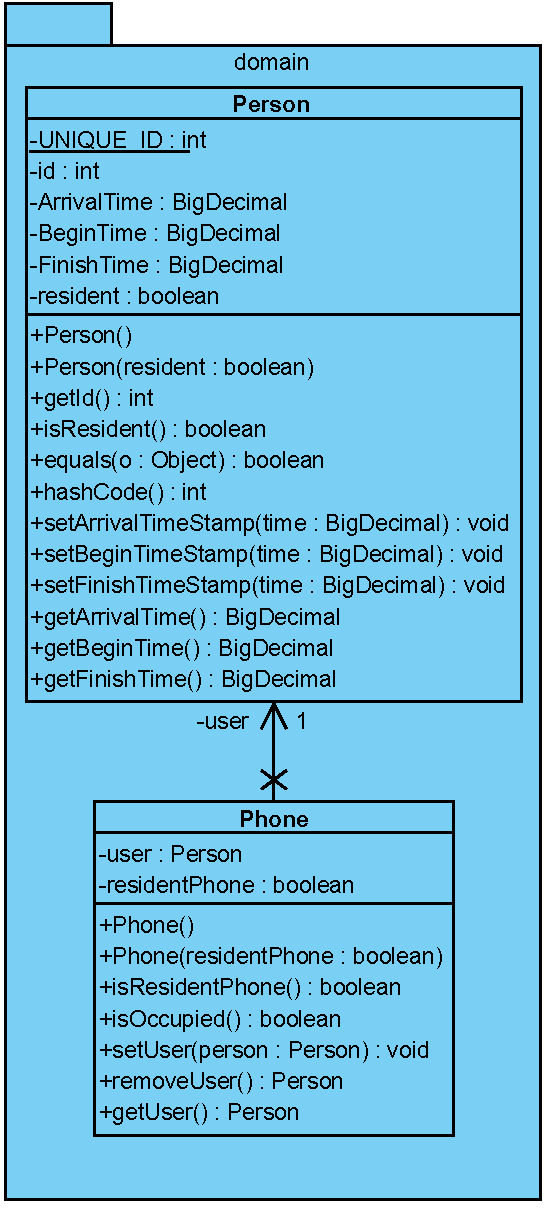
\includegraphics[scale=0.5]{abbildungen/uml/domain.pdf}


\texttt{domain} beschreibt alle notwendigen Datenstrukturen aus der Domäne des Callshops. Hier gibt es Personen und Telefone. Jede neue Person hat eine einzigartige ID und im Laufe der Simulation merkt sie sich ihre persönlichen Zeitpunkte.

Eine Person kann optional ein Resident (Vip) sein. Eine Telefon kann optional nur Residents (VIPs) annehmen.

\subsection{Package calculation, log}

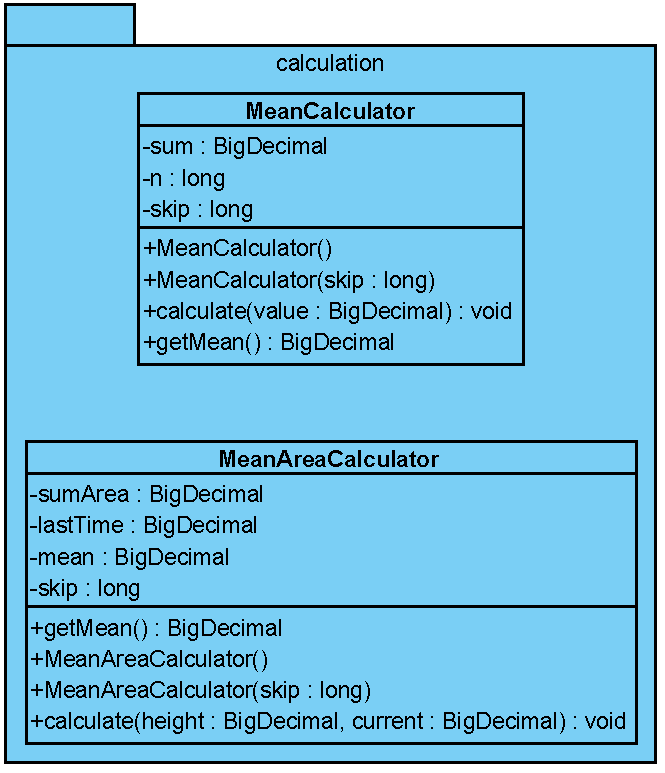
\includegraphics[scale=0.5]{abbildungen/uml/calculation.pdf}
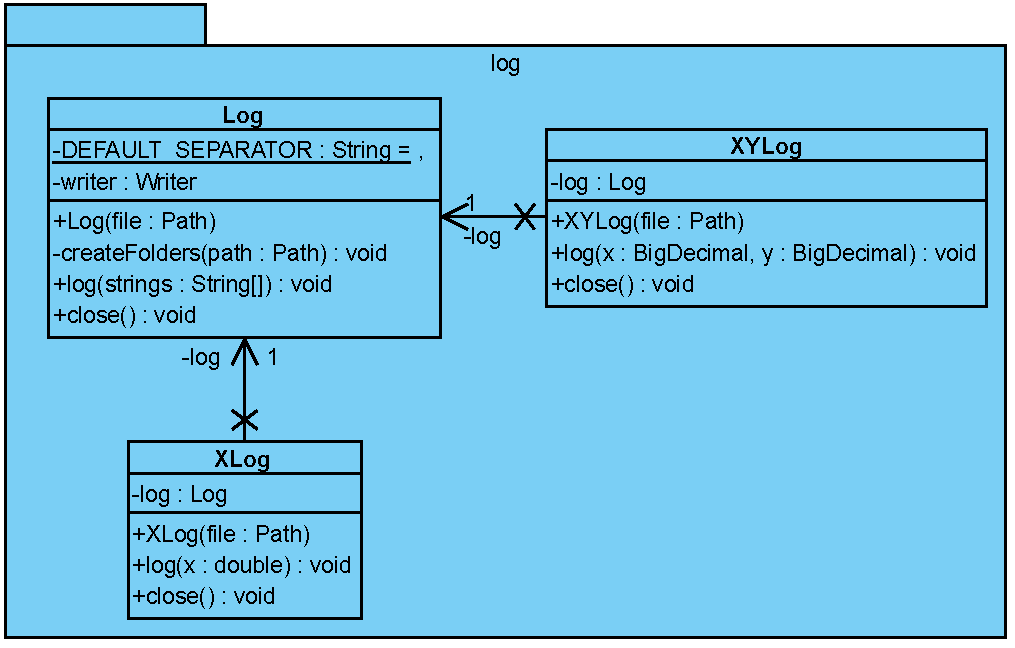
\includegraphics[scale=0.5]{abbildungen/uml/log.pdf}

Die allgemeine Berechnung für Mittelwerte ist in \texttt{calculation} gelöst.
Mit \texttt{log} können Ergebnisse in ein CSV Dokument gespeichert werden.

\subsection{Package config, modellbildung}

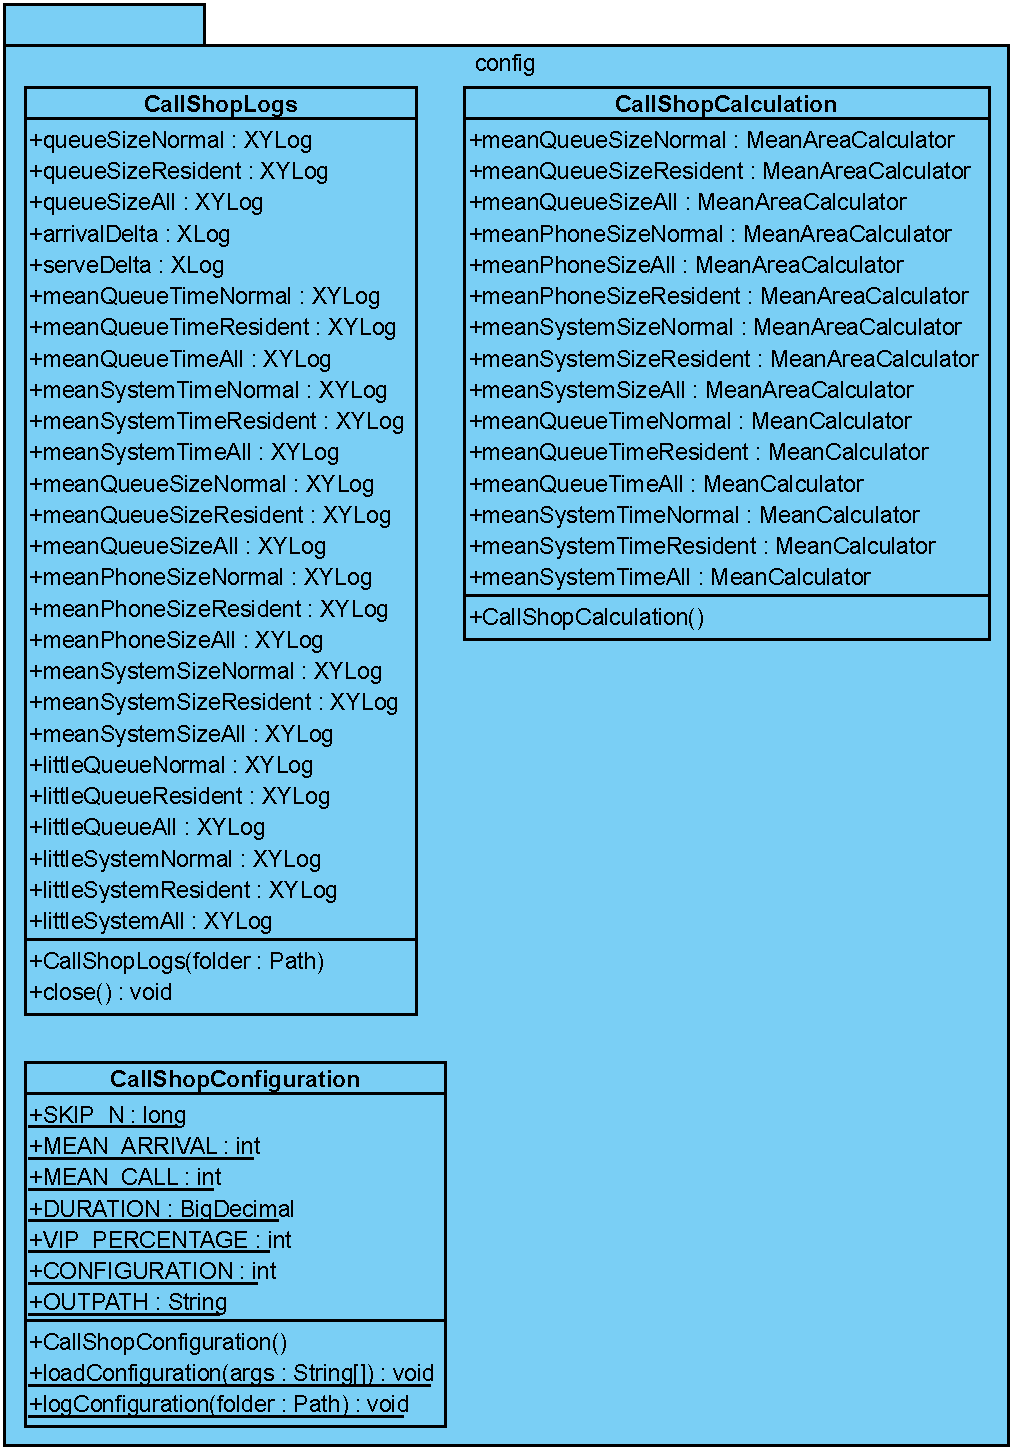
\includegraphics[scale=0.5]{abbildungen/uml/config.pdf}
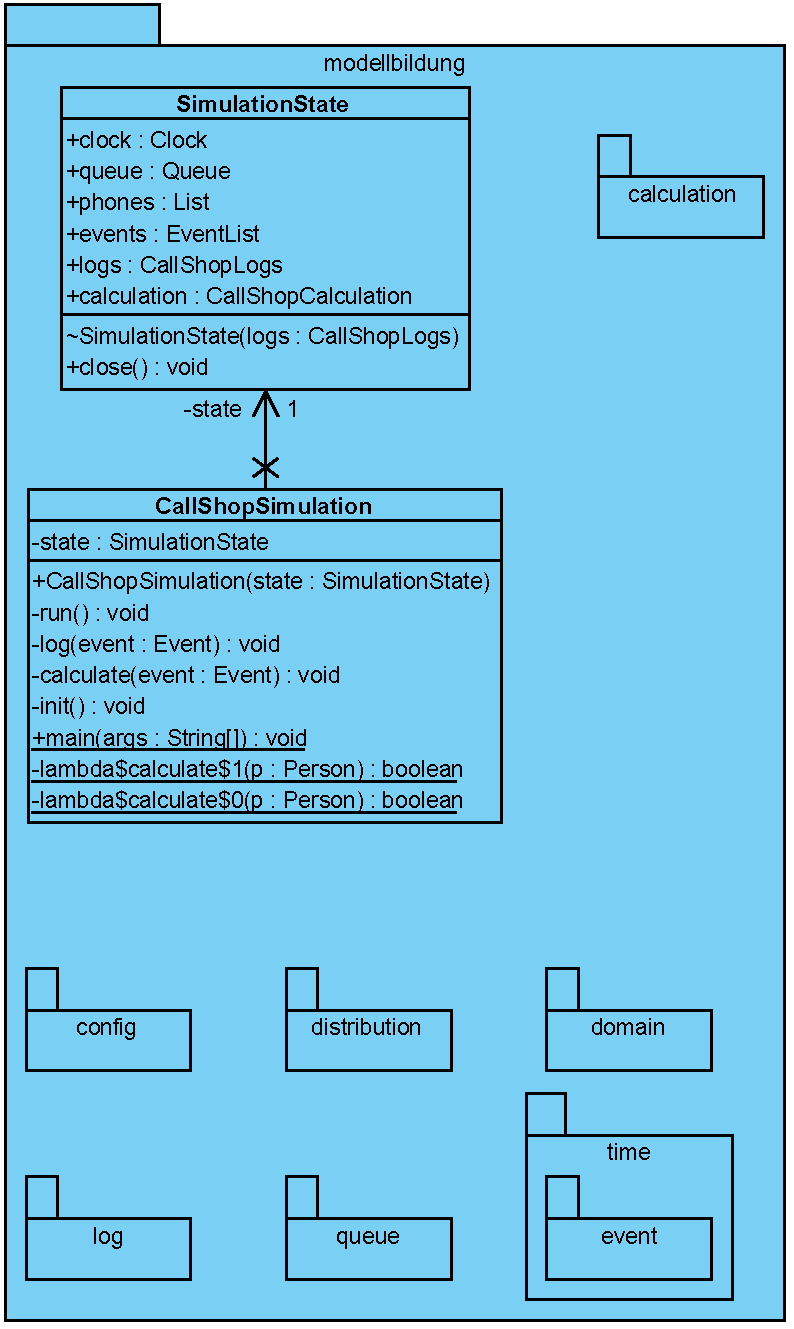
\includegraphics[scale=0.5]{abbildungen/uml/modellbildung.pdf}

In \texttt{config} ist die Konfiguration der Simulation zu finden. Die Logs und Mittelwert-Rechner für die aktuelle konkrete Simulation sind ebenfalls hier definiert.

Das Paket \texttt{modellbildung} beinhaltet alle zuvor beschriebenen Pakete und enthält die Simulationsklasse zum Starten sowie den groben Ablauf der Simulation. Der \texttt{SimulationState} hält den aktuellen Zustand der Simulation.

\section{Überprüfung auf Exponentialverteilung}
Im Zuge dieses Kapitels erfolgt die Überprüfung der, im Zuge der implementierten Simulation, generierten Zufallszahlen. Diese sollen, wie in den Anforderungen definiert, negativ exponentialverteilt sein. \\
Die Überprüfung erfolgt zunächst graphisch mittels eines Histogramms und eines Qunatil-Quantil-Plots. Im Anschluss erfolgt die rechnerische Überprüfung mittels Shapiro-Wilk-, Cramér-von-Mises- und Anderson-Darling-Test.

\subsection{Graphische Überprüfung}

\begin{figure}[htpb]
	\centering
	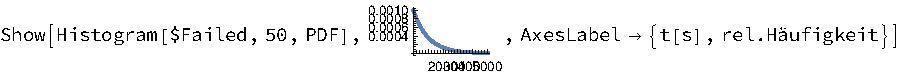
\includegraphics[width=0.8\textwidth]{abbildungen/distribution/histogrammExpVerteilung.pdf}
	\caption{Histogramm der generierten Zufallszahlen}
	\label{fig:HistogrammExp}
\end{figure}

Abbildung \ref{fig:HistogrammExp} zeigt die von der Simulation generierten Zufallszahlen in einem Histogramm. Die blaue Linie stellt den Graph einer Exponentialverteilung dar. Der Verlauf des Histogramms ist nahezu identisch mit dem Verlauf der Exponentialverteilung, was ein Indiz für eine Exponentialverteilung der Daten darstellt.

\begin{figure}[htpb]
	\centering
	\includegraphics[width=0.8\textwidth]{abbildungen/distribution/quantilePlot.pdf}
	\caption{Quantil-Quantil-Diagramm der generierten Zufallszahlen}
	\label{fig:QQPlot}
\end{figure}

In Abbildung \ref{fig:QQPlot} werden die generierten Zufallszahlen in einem Quantil-Quantil-Diagramm dargestellt. Die blaue, gestrichelte Ursprungsgerade zeigt den Verlauf einer Exponentialverteilung im Quantil-Quantil-Diagramm. Die generierten Daten werden durch die blaue Linie repräsentiert. Die Abbildung zeigt somit, dass beide Linien nahezu deckungsgleich sind und es nur eine sehr geringe Abweichung gibt. Das Quantil-Quantil-Diagramm liefert somit einen weiteres Indiz dahingehend, dass die generierten Zufallszahlen tatsächlich exponentialverteilt sind.

\subsection{Rechnerische Überprüfung}
Für eine weitere Überprüfung werden die generierten Daten mittels Shapiro-Wilk-, Cramér-von-Mises- und Anderson-Darling-Test auf eine Exponentialverteilung überprüft. Die Hypothese H0 lautet hierbei: \\
$H_0:$ Die generierten Zufallszahlen sind exponentialverteilt, Signifikanzniveau $\alpha =0,05$ Die Ergebnisse der einzelnen Tests sind in der folgenden Tabelle aufgelistet:
\[\begin{array}{l|ll}
 \text{} & \text{Statistic} & \text{P-Value} \\
\hline
 \text{Anderson-Darling} & 0.482866 & 0.764349 \\
 \text{Cram{\' e}r-von Mises} & 0.0690154 & 0.757621 \\
 \text{Kolmogorov-Smirnov} & 0.00201837 & 0.80994 \\
 \text{Kuiper} & 0.00390365 & 0.478494 \\
 \text{Pearson }\chi ^2 & 191.088 & 0.643726 \\
 \text{Watson }U^2 & 0.0689189 & 0.503982 \\
\end{array}\]



Laut dem Shapiro-Wilk-Test kann die Nullhypothese nicht abgelehnt werden, da der p-Wert mit $0,80994$ deutlich über dem Signifikanzniveau von $0,05$ liegt. Ebenso kann die Nullhypothese bei den Cramér-von-Mises- und Anderson-Darling-Tests nicht abgelehnt werden, da der p-Wert hier ebenso mit $0,764349$ bzw. $0,0764349$ deutlich über dem Signifikanznievau liegt.\\
Durch die Tests kann somit eine Exponentialverteilung der generierten Zufallszahlen nicht wiederlegt werden. In Kombination mit der graphischen Überprüfung ist es plausibel, wenn von exponentialverteilten Werten ausgegangen wird. Ein entgültiger Beweis kann nicht erbracht werden.

\section{Auswertung der Ergebnisse}
Im Zuge dieses Kapitels werden alle Ergebnisse der Simulation und die daraus errechneten Werte erläutert. Zusätzlich werden relevante Größen durch Plots veranschaulicht. Die einzelnen Auswertungen werden mit Hilfe des Theorems von Little validiert.\\
Die Anzahl und damit die Kombinationsmöglichkeiten der unterschiedlichen Parameter ist sehr groß. Im Verlauf dieser Studienarbeit werden ausschließlich die Auswirkungen verschiedene Werte für den Parameter durchschnittliche Zwischenankunftszeit auf den Verlauf der Simulation ausgewertet. Weitere Simulationen mit anderen Parameterwerten können durchgeführt werden. Die unterschiedlichen Parameter sind in der Tabelle \ref{tab:parameter} aufgelistet.


\subsection{Modell \glqq Ein Telefon\grqq}
Für den in Kapitel \ref{requirements} aufgelisteten ersten Betriebsmodus (ein Server, welcher alle Clients bedient) werden im folgenden die Auswertungen aufgeführt. Exemplarisch werden vier verschiedene durchschnittliche Ankunftszeiten für die Clients verwendet. Zunächst wird eine durchschnittliche Ankunftszeit von $1000s$ angenommen, was bei einer durchschnittlichen Telefonierdauer von $100s$ (Dauer der Serverbelegung) einer sehr geringen Serverauslastung entspricht. Anschließend werden mit den durchschnittlichen Ankunftszeiten von $400s$ und $100s$ die Auswirkungen von höherer Serverauslastung auf das Ergebnis der Simulation erläutert. \\

Für jede durchschnittliche Ankunftszeit werden zunächst die zu erwartenden Werte, basierend auf den Formeln für M/M/1 Warteschlangenmodelle ermittelt. Die einzelnen Formeln sind im folgenden Kapitel aufgeführt. Betrachtet werden hierbei, wie in den \ref{requirements} erläutert die durchschnittliche Anzahl von Kunden im System, durchschnittliche Warteschlangenlänge, durchschnittliche Verweildauer im System und die durchschnittliche Verweildauer in der Warteschlange. Die berechneten Größen werden als Erwartungswerte betrachtet gegen die die durch die Simulation ermittelten Werte geprüft werden.

Die Maßnahmen für die Verifikation der implementierten Simulation werden im Kapitel (REFERENZ AUF DIE UNITTEST KAPITEL) näher beschrieben. In den folgenden Abbildungen wird die durchschnittliche Zwischenankunftszeit mit \glqq MeanAr\grqq abgekürzt.

\subsubsection{Formeln für M/M/1 Warteschlangenmodelle}
\label{Formeln}
Die im folgenden aufgeführten Formeln gelten für M/M/1 Warteschlangenmodelle im eingeschwungenen Zustand. Mit $Ls$ wird die durchschnittliche Anzahl von Kunden im System bezeichnet. $Lq$ gibt die durchschnittliche Länge der Warteschlange an. $Ws$ definiert die durchschnittliche Verweildauer der einzelnen Kunden im System und $Wq$ die durchschnittliche Verweildauer in der Warteschlange.

\begin{equation}
Ls=\frac{\lambda}{\mu - \lambda}
\end{equation}
\begin{equation}
Lq=\frac{\rho\lambda}{\mu - \lambda}
\end{equation}
\begin{equation}
Ws=\frac{1}{\mu - \lambda}
\end{equation}
\begin{equation}
Wq=\frac{\rho}{\mu - \lambda}
\end{equation}

In den einzelnen Gleichungen sind $\lambda$, $\mu$ und $\rho$ wie folgt definiert: $\lambda$ beschreibt die durchschnittliche Ankunftszeit der Kunden pro Sekunde. $\mu$ definiert die durchschnittliche Telefonierdauer der Kunden pro Sekunde. Und $\rho$ beschreibt die durchschnittliche Auslastung des Telefons \cite{MM1Formeln}.

\begin{equation}
\rho=\frac{\lambda}{\mu}
\end{equation}

\subsubsection{Validierung der einzelnen Auswertung auf Basis des Little Theorems}
Laut dem Theorem von Little muss die durchschnittliche Anzahl von Kunden in einem Warteschlangensystem gleich dem Produkt aus der durchschnittlichen Ankunftsrate ($\Lambda$) und der durchschnittlichen Verweildauer ($Ws$) im System sein, wenn das System sich in einem eingeschwungenen Zustand befindet.

\begin{equation}
Ls=\lambda*Ws
\end{equation}

Stellt man die Formel um, muss im eingeschwungenen Zustand gelten:

\begin{equation}
\label{eq:little}
\lambda*Ws - Ls=0
\end{equation}

Anhand dieser Gleichung werden im weiteren Verlauf der Studienarbeit die einzelnen Auswertungen validiert.

\subsubsection{Durchschnittliche Zwischenankunftszeit der Clients: $1000s$}

\paragraph{Theoretische Erwartungswerte laut M/M/1 Warteschlangenmodell}
\\
Bei einer durchschnittlichen Zwischenankunftszeit von $1000s$ ($\lambda=\frac{1}{1000}$, $\mu=\frac{1}{100}$)ergeben sich, basierend auf den in Abschnitt \ref{Formeln} aufgeführten Formeln, folgende Erwartungswerte:
\begin{equation}
Ls=0,111111
\end{equation}
\begin{equation}
Lq=0,0111111
\end{equation}
\begin{equation}
Ws=111,111
\end{equation}
\begin{equation}
Wq=11,1111
\end{equation}
Die einzelnen Erwartungswerte sind in den nachfolgenden Abbildungen durch eine gelbe Linie hervorgehoben.

\paragraph{Verwendung der implementierten Java-Simulation, Berechnung in Java}
\label{JavaOnePhone1000}
\\
\begin{figure}[htpb]
	\centering
	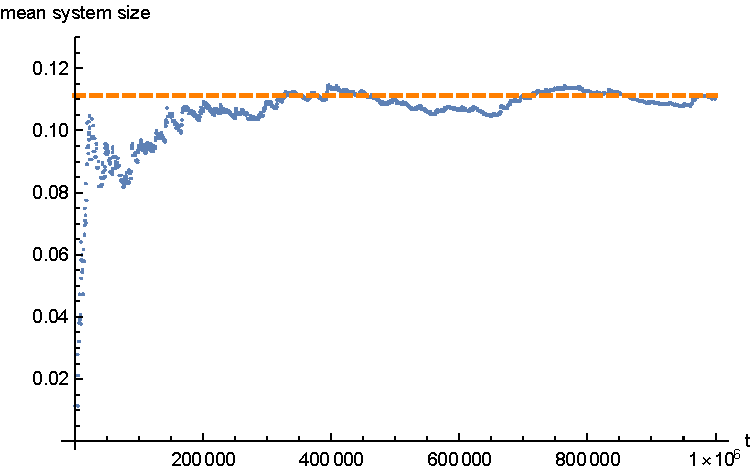
\includegraphics[width=0.8\textwidth]{abbildungen/1_Phone/Arrival_1000_Serve_100_dur_1000000_Skip_0/MeanSystemSize.pdf}
	\caption{Durchschnittliche Anzahl an Kunden im System, MeanAr = $1000s$}
	\label{fig:meanSystemSize1000}
\end{figure}

Abbildung \ref{fig:meanSystemSize1000} zeigt die durchschnittliche Anzahl an Kunden im System an. Ab einer Simulationszeit von ca $200000s$ liegt diese durchschnittlich bei $0.11$, schwankt jedoch bis zum Ende der Simulation um ca. $0,01$. Der Erwartungswert von $0,111111$ wird durch die Simulation nicht exakt erreicht. Ursache hierfür könnte ein systematischen Fehler, beispielsweise aufgrund von Rundungsfehlern, von ca. $0,01$ bei der Berechnung sein. Alternativ würde ein noch nicht vollständig eingeschwungenes System das Verhalten ebenfalls erklären. Weitere Erkenntnisse liefert die Validierung mit Hilfe des Little Theorems. Allgemein zeigt dieser Plot, dass die durchschnittliche Anzahl an Kunden im System sehr gering ist. Durch die Vergleichsweise kurze Telefonierzeit in Kombination mit einer lange Zwischenankunftszeit ist dieser Wert plausibel.

\begin{figure}[htpb]
	\centering
	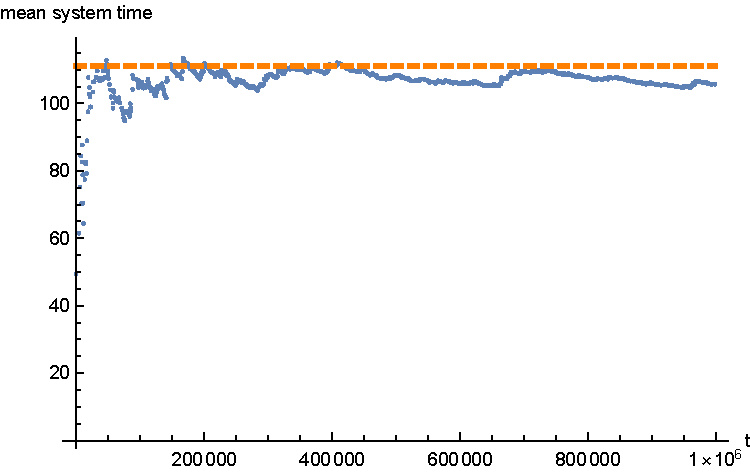
\includegraphics[width=0.8\textwidth]{abbildungen/1_Phone/Arrival_1000_Serve_100_dur_1000000_Skip_0/MeanSystemTime.pdf}
	\caption{Durchschnittliche Verweildauer der Kunden im System, MeanAr = $1000s$}
	\label{fig:meanSystemTime1000}
\end{figure}

Betrachtet man Abbildung \ref{fig:meanSystemTime1000}, wird deutlich, dass die durchschnittliche Verweilsdauer im System bis zu einer Simulationszeit von $200000s$ stark variiert. Doch auch mit steigender Simulationszeit bleibt sie unter dem erwarteten Wert von $111.111$ bei durchschnittlich. Der Grund hierfür könnte wiederum ein systematischer Fehler in der Berechnung, beispielsweise aufgrund von Ungenauigkeiten durch Runden sein, oder ein noch nicht vollständig eingeschwungenes System.

\begin{figure}[htpb]
	\centering
	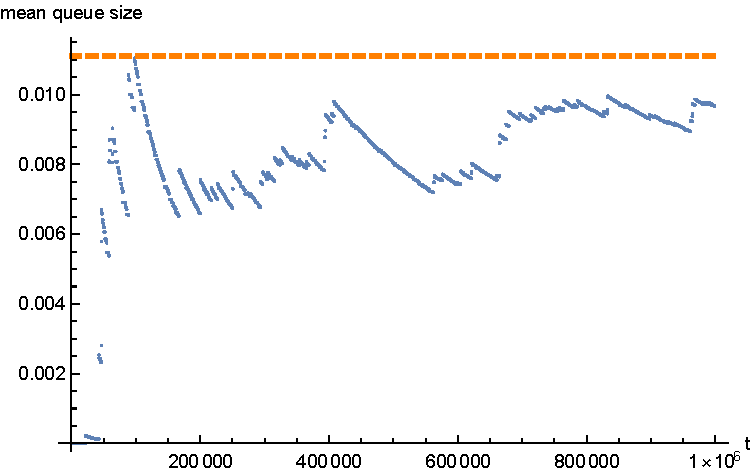
\includegraphics[width=0.8\textwidth]{abbildungen/1_Phone/Arrival_1000_Serve_100_dur_1000000_Skip_0/MeanQueueSize.pdf}
	\caption{Durchschnittliche Warteschlangenlänge, MeanAr = $1000s$}
	\label{fig:meanQueueSize1000}
\end{figure}

Bei der Betrachtung der in Abbildung \ref{fig:meanQueueSize1000} gezeigte durchschnittliche Warteschlangenlänge fällt auf, dass die Werte wiederum bis zu einer Simulationsdauer von $200000s$ stark variieren schwanken. Anschließend nähern sich die Werte dem dem Erwartungswert von $0,0111111$ an, bleiben jedoch unterhalb. Es handelt sich hierbei um eine Abweichung von ca. $0,0015$. Ursache dafür könnte, wie bereits erwähnt ein systematischen Fehler, oder ein nicht vollständig eingeschwungenes System sein.

\begin{figure}[htpb]
	\centering
	\includegraphics[width=0.8\textwidth]{abbildungen/1_Phone/Arrival_1000_Serve_100_dur_1000000_Skip_0/MeanQueueTime.pdf}
	\caption{Durchschnittliche Verweildauer in der Warteschlange , MeanAr = $1000s$}
	\label{fig:meanQueueTime1000}
\end{figure}

Die in Abbildung \ref{fig:meanQueueTime1000} aufgeführte durchschnittliche Verweildauer in der Warteschlange weißt einen ähnlichen Verlauf auf wie die in Abbildung \ref{fig:meanQueueSize1000} gezeigte durchschnittliche Warteschlangenlänge. Dieses Verhalten ist plausibel, da bei einer größeren Warteschlangenlänge auch die Wartezeit in der Warteschlange steigt. Gegen Ende der Simulation näher sich die durchschnittliche Verweildauer in der Warteschlange dem Erwartungswert von $11,1111$ an, bleibt jedoch mit einer Abweichung von ca. $1,51$ unterhalb.

\begin{figure}[htpb]
	\centering
	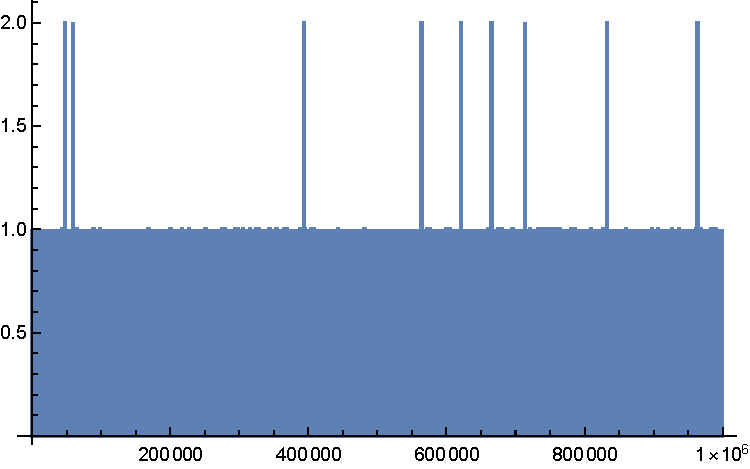
\includegraphics[width=0.8\textwidth]{abbildungen/1_Phone/Arrival_1000_Serve_100_dur_1000000_Skip_0/QueueStepPlotAll.pdf}
	\caption{Warteschlangenlänge (ungefiltert) , MeanAr = $1000s$}
	\label{fig:QueueStepPlotAll1000}
\end{figure}
\begin{figure}[htpb]
	\centering
	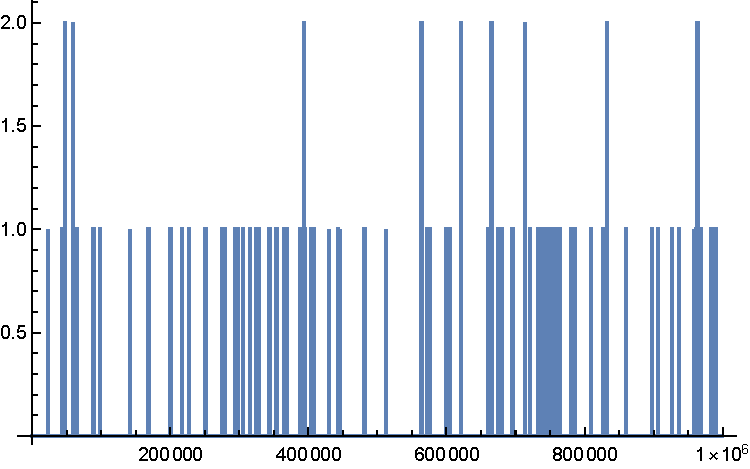
\includegraphics[width=0.8\textwidth]{abbildungen/1_Phone/Arrival_1000_Serve_100_dur_1000000_Skip_0/QueueStepPlotAllFiltered.pdf}
	\caption{Warteschlangenlänge (gefiltert) , MeanAr = $1000s$}
	\label{fig:QueueStepPlotAllFiltered1000}
\end{figure}

Die Abbildung \ref{fig:QueueStepPlotAll1000} zeigt die einzelnen Werte für die Warteschlangenlänge über die Simulationszeit. Diese Abbildung ist nicht aussagekräftig. Hintergrund dafür ist die Implementierung der Simulation. Im Warteschlangenmodell wird zwischen drei verschiedenen Events unterschieden. Betritt ein neuer Kunde den Telefonshop, wird ein Arrival Event ausgelöst und die Warteschlangenlänge wird um 1 erhöht. Ist das Telefon frei, wird ein Begin Event ausgelöst und die Warteschlangenlänge wird um 1 reduziert. Hat ein Kunde sein Telefonat beendet, wird ein Finish Event ausgelöst, was wiederum ein Begin Event auslöst, da das Telefon frei ist. Ein Problem gibt es hierbei für den Fall, dass kein Kunde im Laden steht und somit auch die Warteschlange leer und das Telefon frei ist. Betritt nun ein neuer Kunde den Laden, wird ein Arrival Event ausgelöst und direkt anschließend ein Begin Event, da das Telefon frei ist und der Kunde sein Telefonat sofort beginnen kann. Er befindet sich somit für $0s$ in der Warteschlange. Aufgrund der Events wird die Warteschlangenlänge jedoch trotzdem erhöht und direkt wieder gesenkt. Es gibt somit für den gleichen Zeitstempel zwei unterschiedliche Warteschlangenlängen. Abbildung \ref{fig:QueueStepPlotAllFiltered1000} zeigt die gleiche Situation ohne die eben erläuterte Situation. Es wird hierbei nur eine Warteschlangenlänge angezeigt, wenn auch wirklich ein Kunde länger als $0s$ in der Warteschlange wartet. Da das System nur sehr gering ausgelastet ist, ist die geringe Warteschlangenlänge plausibel.\\

\paragraph{Validierung der Simulation}
\\
\begin{figure}[htpb]
	\centering
	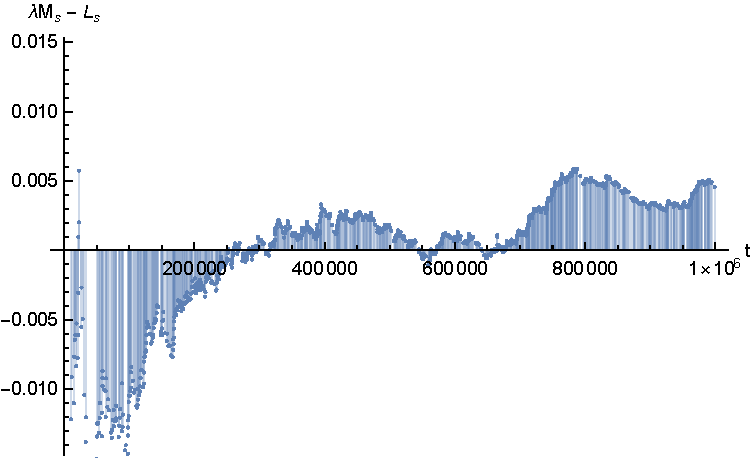
\includegraphics[width=0.8\textwidth]{abbildungen/1_Phone/Arrival_1000_Serve_100_dur_1000000_Skip_0/LittleSystem.pdf}
	\caption{Darstellung der Differenz: $\lambda * Ws - Ls$ über die Simulationszeit (Little Theorem)}
	\label{fig:LittleSystem1000}
\end{figure}

In Abbildung \ref{fig:LittleSystem1000} ist der Verlauf der Gleichung \ref{eq:little} über die Simulationszeit aufgeführt. Ab einer Simulationsdauer von ca. $350000s$ liegt der Wert sehr nach an dem geforderten Erwartungswert von $0$, schwankt jedoch bis zum Ende der Simulation im Bereich von $0,004$. Da die Differenz zum Erwartungswert sehr gering ist, liegt die Ursache für diese Abweichung vermutlich in Ungenauigkeiten bei der Berechung der Werte. Die durchschnittliche Anzahl an Kunden im System wird entweder um $0,004$ zu gering angenommen, oder die Verweildauer der Kunden im System um $0,004$ zu lang. Ebenso ist eine Kombination der beiden Fehler möglich. Insgesamt deckt sich diese Aussage mit den Abweichungen in den einzelnen Abbildungen.

Abschließend sind im folgenden die von der implementierten Simulation berechneten Werte für die durchschnittliche Warteschlangenlänge, Wartezeit in der Warteschlange, Anzahl an Clients im System und Zeit im System im Vergleich zu den entsprechenden theoretisch errechneten Werten (für ein eingeschwungenes System) aufgelistet:
\[\begin{array}{cc}
 \text{mean queue size} & 0.00537307572764891636692565082375430880024384373 \\
 \text{mean queue time} & 8.19291 \\
 \text{mean system size} & 0.06921258430823697932263116253494454280311475015 \\
 \text{mean system time} & 105.458 \\
\end{array}\]



Alle vier ermittelten Durchschnittswerte liegen, ab einer Simulationsdauer von ca. $400000s$ sehr nah an den Werten, welche für ein eingeschwungenes Warteschlangensystem errechnet wurden. Da auch das in Abbildung  \ref{fig:LittleSystem1000} ersichtliche Ergebnis der Differenz zeigt, dass das System ab einer Simulationszeit von ca. $400000s$ den für ein eingeschwungenes System erforderlichen Wert von $0$ näherungsweise erreicht, kann somit davon ausgegangen werden, dass der Steady State (eingeschwungene Zustand) bei dieser Simulationsdauer erreicht wurde.

\subsubsection{Durchschnittliche Zwischenankunftszeit der Clients: $400s$}
\paragraph{Theoretische Erwartungswerte laut M/M/1 Warteschlangenmodell}
\label{FormenlnMM1}
\\
Bei einer durchschnittlichen Zwischenankunftszeit von $400s$ ($\lambda=\frac{1}{400}$, $\mu=\frac{1}{100}$)ergeben sich, basierend auf den in Abschnitt \ref{Formeln} aufgeführten Formeln, folgende Erwartungswerte:
\begin{equation}
Ls=0,333333
\end{equation}
\begin{equation}
Lq=0,0833333
\end{equation}
\begin{equation}
Ws=133,333
\end{equation}
\begin{equation}
Wq=33,3333
\end{equation}
Die einzelnen Erwartungswerte sind in den nachfolgenden Abbildungen durch eine gelbe Linie hervorgehoben.

\paragraph{Verwendung der implementierten Java-Simulation, Berechnung in Java}
\\
\begin{figure}[htpb]
	\centering
	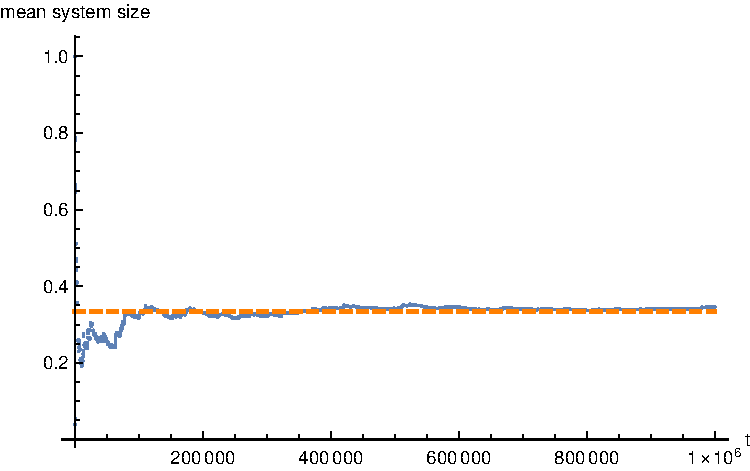
\includegraphics[width=0.8\textwidth]{abbildungen/1_Phone/Arrival_400_Serve_100_dur_1000000_Skip_0/MeanSystemSize.pdf}
	\caption{Durchschnittliche Anzahl an Kunden im System, MeanAr = $400s$}
	\label{fig:meanSystemSize400}
\end{figure}

Abbildung \ref{fig:meanSystemSize400} zeigt die durchschnittliche Anzahl an Kunden im System an. Ab einer Simulationszeit von ca $400000s$ schwankt diese nur noch sehr gering, liegt jedoch über dem Erwartungswert von $0,333333$. Es ist von einem systematischen Fehler von $0,01$, oder einem nicht vollständig eingeschwungenen System auszugehen.

\begin{figure}[htpb]
	\centering
	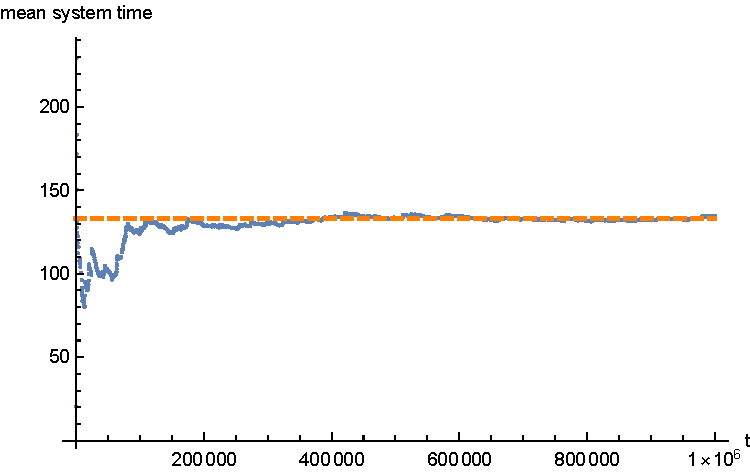
\includegraphics[width=0.8\textwidth]{abbildungen/1_Phone/Arrival_400_Serve_100_dur_1000000_Skip_0/MeanSystemTime.pdf}
	\caption{Durchschnittliche Verweildauer der Kunden im System, MeanAr = $400s$}
	\label{fig:meanSystemTime400}
\end{figure}

Auch die in Abbildung \ref{fig:meanSystemTime400} dargestellte durchschnittliche Verweildauer im System schwankt bis zu einer Simulationsdauer von ca. $400000s$ stark. Anschließend schwankt sie um ca. $2$ um den erwarteten Wert von $133,333$.

\begin{figure}[htpb]
	\centering
	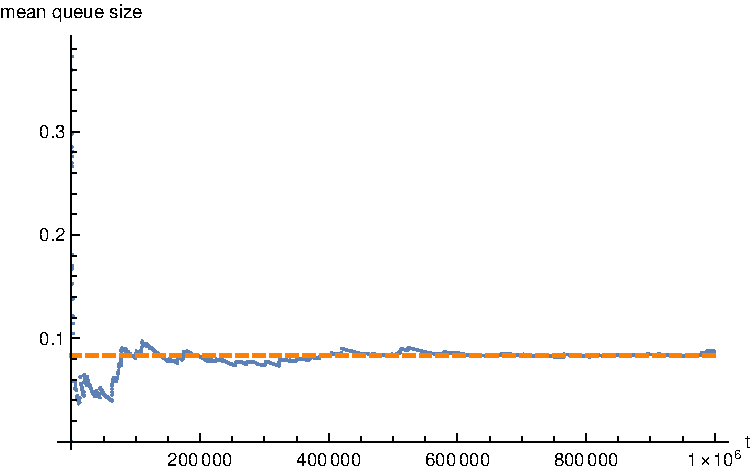
\includegraphics[width=0.8\textwidth]{abbildungen/1_Phone/Arrival_400_Serve_100_dur_1000000_Skip_0/MeanQueueSize.pdf}
	\caption{Durchschnittliche Warteschlangenlänge, MeanAr = $400s$}
	\label{fig:meanQueueSize400}
\end{figure}

Die in Abbildung \ref{fig:meanQueueSize400} gezeigte durchschnittliche Warteschlangenlänge schwankt ebenso ab einer Simulationsdauer von ca. $400000s$ nur noch um ca. $0,001$ um den erwarteten Wert von $0,0833333$.

\begin{figure}[htpb]
	\centering
	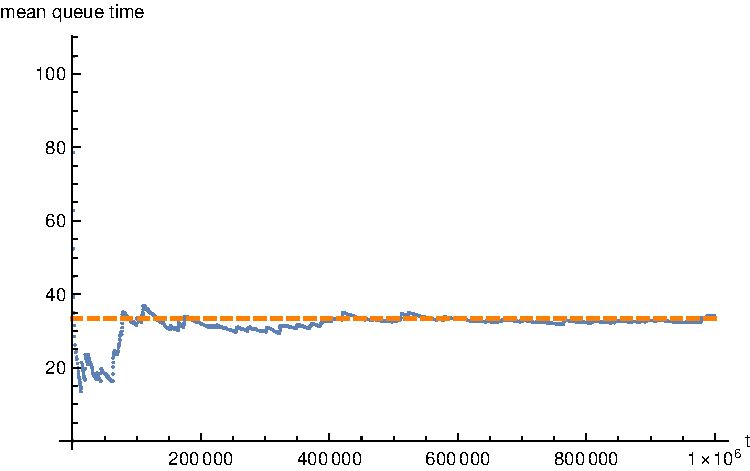
\includegraphics[width=0.8\textwidth]{abbildungen/1_Phone/Arrival_400_Serve_100_dur_1000000_Skip_0/MeanQueueTime.pdf}
	\caption{Durchschnittliche Verweildauer in der Warteschlange , MeanAr = $400s$}
	\label{fig:meanQueueTime400}
\end{figure}

Die in Abbildung \ref{fig:meanQueueTime400} aufgeführte durchschnittliche Verweildauer in der Warteschlange weißt einen ähnlichen Verlauf auf wie die in Abbildung \ref{fig:meanQueueSize400} gezeigte durchschnittliche Warteschlangenlänge. Dieses Verhalten ist plausibel, da bei einer größeren Warteschlangenlänge auch die Wartezeit in der Warteschlange steigt. Beide Werte schwanken ab einer Simulationsdauer von ca. $400000s$ um den Erwartungswert. Die durchschnittliche Verweildauer in der Warteschlange schwankt um ca. $2$ um den Erwartungswert von $33,3333$.

\begin{figure}[htpb]
	\centering
	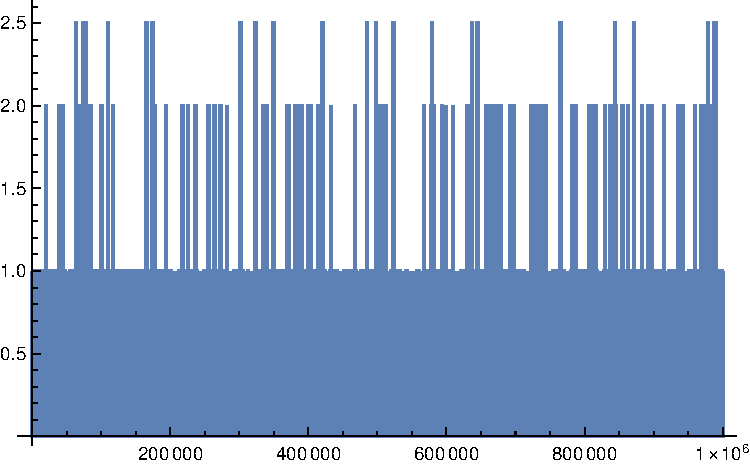
\includegraphics[width=0.8\textwidth]{abbildungen/1_Phone/Arrival_400_Serve_100_dur_1000000_Skip_0/QueueStepPlotAll.pdf}
	\caption{Warteschlangenlänge (ungefiltert) , MeanAr = $400s$}
	\label{fig:QueueStepPlotAll400}
\end{figure}
\begin{figure}[htpb]
	\centering
	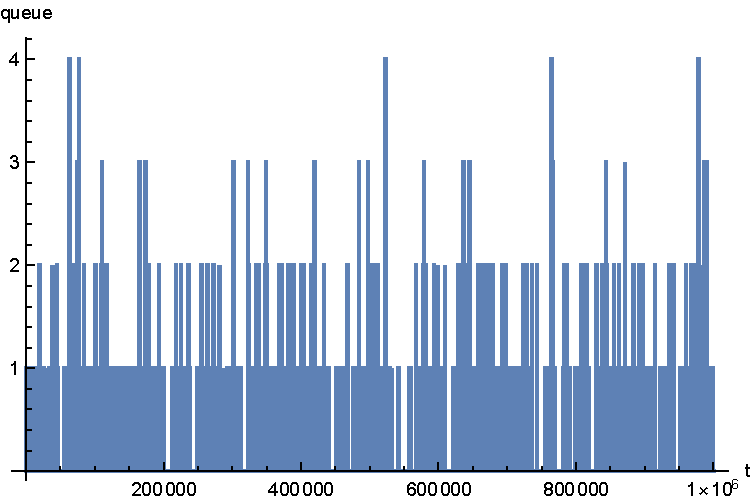
\includegraphics[width=0.8\textwidth]{abbildungen/1_Phone/Arrival_400_Serve_100_dur_1000000_Skip_0/QueueStepPlotAllFiltered.pdf}
	\caption{Warteschlangenlänge (gefiltert) , MeanAr = $400s$}
	\label{fig:QueueStepPlotAllFiltered400}
\end{figure}

Abschließend sind in den Abbildungen \ref{fig:QueueStepPlotAll400} und \ref{fig:QueueStepPlotAllFiltered400} jeweils die Länge der Warteschlange dargestellt. Aufgrund des in \ref{JavaOnePhone1000} erläuterten Problems mit der Inkrementierung bzw. Dekrementierung der Warteschlangenlänge bei den einzelnen Events, ist die tatsächliche Länge in der Abbildung \ref{fig:QueueStepPlotAllFiltered400} gefiltert besser zu sehen. Die Warteschlangenlänge ist größer als bei einer durchschnittlichen Zwischenankunftszeit von $1000s$, doch das Telefon ist noch nicht zu voll ausgelastet, da die Warteschlangenlänge phasenweise noch immer $0$ ist.


\paragraph{Validierung der Simulation}
\\
\begin{figure}[htpb]
	\centering
	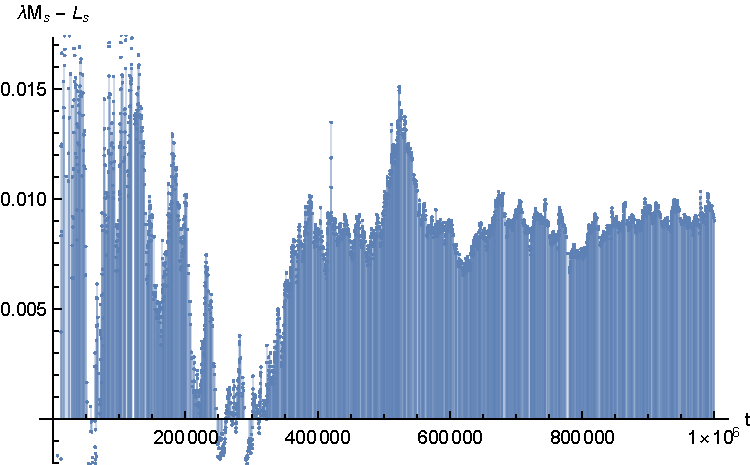
\includegraphics[width=0.8\textwidth]{abbildungen/1_Phone/Arrival_400_Serve_100_dur_1000000_Skip_0/LittleSystem.pdf}
	\caption{Darstellung der Differenz: $\lambda * Ws - Ls$ über die Simulationszeit (Little Theorem)}
	\label{fig:LittleSystem400}
\end{figure}

In Abbildung \ref{fig:LittleSystem400} ist der Verlauf der Gleichung \ref{eq:little} über die Simulationszeit aufgeführt. Ab einer Simulationsdauer von ca. $400000s$ schwankt der Wert nur noch geringfügig. Die Werte liegen jedoch bis zum Ende der Simulation bei durchschnittlich ca. $0,009$. Wie auch bei der Auswertung der Simulation mit einer durchschnittlichen Zwischenankunftszeit von $1000s$, kann hier wiederum von einem systematischen Fehler von $0,009$ mit den selben Ursachen ausgegangen werden. Die Abweichung ist hier größer, da aufgrund der niedrigeren Zwischenankunftszeit deutlich mehr Kunden den Laden besucht haben und somit mehr Zeiten verrechnet wurden. Insgesamt deckt sich dieser Fehler mit den Abweichungen in den einzelnen Abbildungen.

Abschließend sind im folgenden die von der implementierten Simulation berechneten Werte für die durchschnittliche Warteschlangenlänge, Wartezeit in der Warteschlange, Anzahl an Clients im System und Zeit im System im Vergleich zu den entsprechenden theoretisch errechneten Werten (für ein eingeschwungenes System) aufgelistet:
\[\begin{array}{cc}
 \text{mean queue size} & 0.00537307572764891636692565082375430880024384373 \\
 \text{mean queue time} & 8.19291 \\
 \text{mean system size} & 0.06921258430823697932263116253494454280311475015 \\
 \text{mean system time} & 105.458 \\
\end{array}\]



Alle vier ermittelten Durchschnittswerte liegen, ab einer Simulationsdauer von ca. $400000s$ sehr nah an den Werten, welche für ein eingeschwungenes Warteschlangensystem errechnet wurden. Das in Abbildung  \ref{fig:LittleSystem400} ersichtliche Ergebnis der Differenz zeigt, dass das System, abgesehen vom erläuterten systematischen Fehler, ab einer Simulationszeit von ca. $600000s$ der für ein eingeschwungenes System erforderliche Wert von $0$ näherungsweise erreicht wird. Es kann somit davon ausgegangen werden, dass der Steady State (eingeschwungene Zustand) ab einer Simulationsdauer von $600000s$ erreicht wurde.

\subsubsection{Durchschnittliche Ankunftszeit der Clients: $100s$}
\paragraph{Theoretische Erwartungswerte laut M/M/1 Warteschlangenmodell}
\\
Für durchschnittliche Zwischenankunftszeit und durchschnittliche Telefonierdauer $100s$ ($\lambda=\frac{1}{100}$, $\mu=\frac{1}{100}$), lassen sich die durchschnittliche Warteschlangenlänge, Wartezeit in der Warteschlange, Anzahl an Clients im System und Zeit im System nicht berechnen. Die Warteschlangenlänge steigt aufgrund der zu hohen Auslastung des Telefons gegen unendlich. Somit steigt auch die durchschnittliche Anzahl an Kunden im System gegen unendlich, da diese sich aus den Kunden in der Warteschlange und dem Kunden am Telefon zusammensetzt. Bei einer unendlich langen Warteschlange ist folglich auch die Wartezeit unendlich lang. Außerdem folgt aus einer unendlichen Anzahl von Kunden im System auch, dass die durchschnittliche Zeit im System unendlich lang wird.

\paragraph{Verwendung der implementierten Java-Simulation, Berechnung in Java}

\begin{figure}[htpb]
	\centering
	\includegraphics[width=0.8\textwidth]{abbildungen/1_Phone/Arrival_100_Serve_100_dur_1000000_Skip_0/MeanSystemSize.pdf}
	\caption{Durchschnittliche Anzahl an Kunden im System, MeanAr = $100s$}
	\label{fig:meanSystemSize100}
\end{figure}

Abbildung \ref{fig:meanSystemSize100} zeigt die durchschnittliche Anzahl an Kunden im System an. Durch die großen Schwankungen kann nicht von einem eingeschwungenen System ausgegangen werden. Für eine genauere Beurteilung müsste die Simulation hierfür mit einer längeren Simulationsdauer erneut durchgeführt werden. Ob die durchschnittliche Anzahl der Kunden an Kunden im System gegen den erwarteten Wert von unendlich steigt, kann erst dann analysiert werden.

\begin{figure}[htpb]
	\centering
	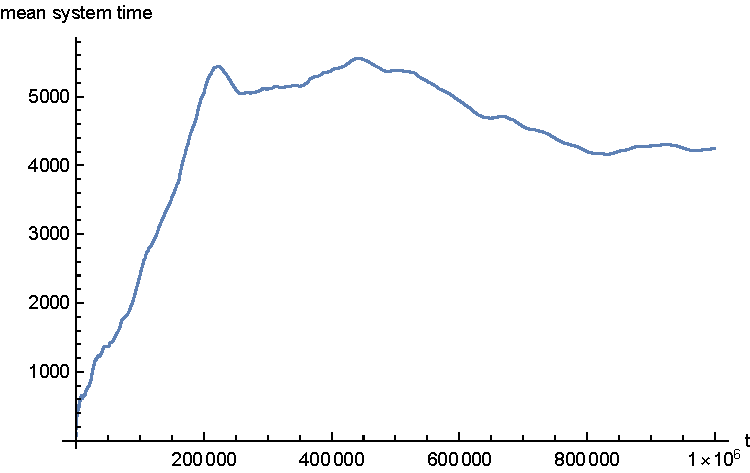
\includegraphics[width=0.8\textwidth]{abbildungen/1_Phone/Arrival_100_Serve_100_dur_1000000_Skip_0/MeanSystemTime.pdf}
	\caption{Durchschnittliche Verweildauer der Kunden im System, MeanAr = 100}
	\label{fig:meanSystemTime100}
\end{figure}

Abbildung \ref{fig:meanSystemTime100} zeigt die durchschnittliche Verweildauer der Kunden im System. Wiederum kann davon ausgegangen werden, dass das System noch nicht eingeschwungen war, bzw. nicht einschwingen wird.

\begin{figure}[htpb]
	\centering
	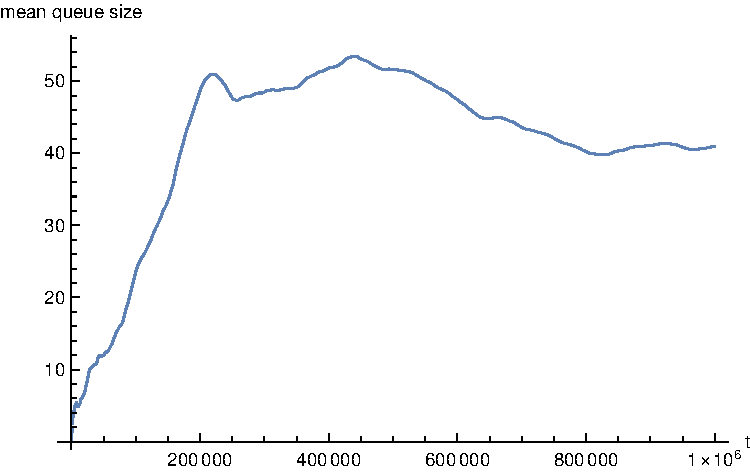
\includegraphics[width=0.8\textwidth]{abbildungen/1_Phone/Arrival_100_Serve_100_dur_1000000_Skip_0/MeanQueueSize.pdf}
	\caption{Durchschnittliche Warteschlangenlänge, MeanAr = 100}
	\label{fig:meanQueueSize100}
\end{figure}

Die Abbildungen \ref{fig:meanQueueSize100} und \ref{fig:meanQueueTime100} und auch weisen einen ähnlichen Verlauf auf wie \ref{fig:meanSystemTime100}. Die Werte schwanken ebenfalls bis zum Ende der Simulation stark.

\begin{figure}[htpb]
	\centering
	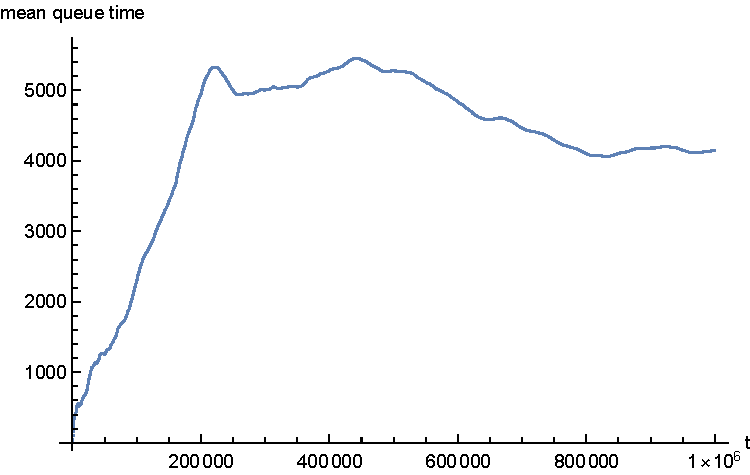
\includegraphics[width=0.8\textwidth]{abbildungen/1_Phone/Arrival_100_Serve_100_dur_1000000_Skip_0/MeanQueueTime.pdf}
	\caption{Durchschnittliche Verweildauer in der Warteschlange , MeanAr = 100}
	\label{fig:meanQueueTime100}
\end{figure}

Abschließend sind in den Abbildungen \ref{fig:QueueStepPlotAll100} und \ref{fig:QueueStepPlotAllFiltered100} jeweils die Länge der Warteschlange dargestellt. Aufgrund des in \ref{JavaOnePhone1000} erläuterten Problems mit der Inkrementierung bzw. Dekrementierung der Warteschlangenlänge bei den einzelnen Events, zeigt Abbildung \ref{fig:QueueStepPlotAllFiltered400} wiederum die gefilterten Werte. Die Werte in beiden Abbildungen schwanken jedoch so stark, dass kein Unterschied mehr ersichtlich ist. Gegen Ende der Simulation steigen die Werte deutlich an. Ob sie gegen den erwarteten Wert von unendlich ansteigen lässt sich nur im Zuge einer erneuten Simulation mit einer längeren Simulationsdauer ermitteln.

\begin{figure}[htpb]
	\centering
	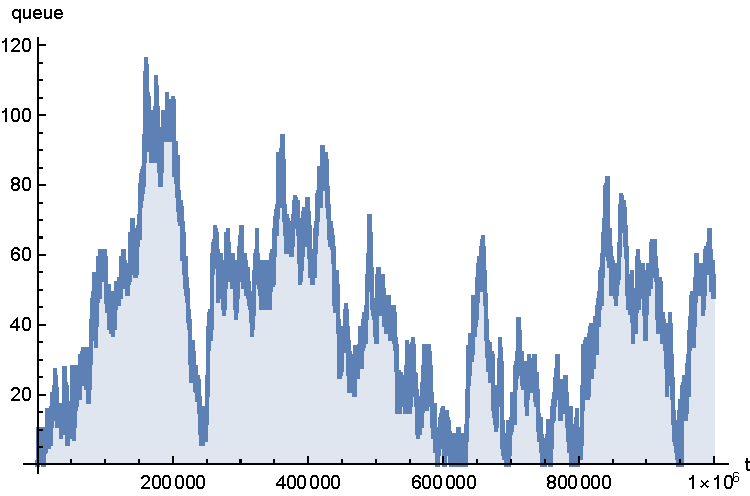
\includegraphics[width=0.8\textwidth]{abbildungen/1_Phone/Arrival_100_Serve_100_dur_1000000_Skip_0/QueueStepPlotAll.pdf}
	\caption{Warteschlangenlänge (ungefiltert) , MeanAr = 100}
	\label{fig:QueueStepPlotAll100}
\end{figure}
\begin{figure}[htpb]
	\centering
	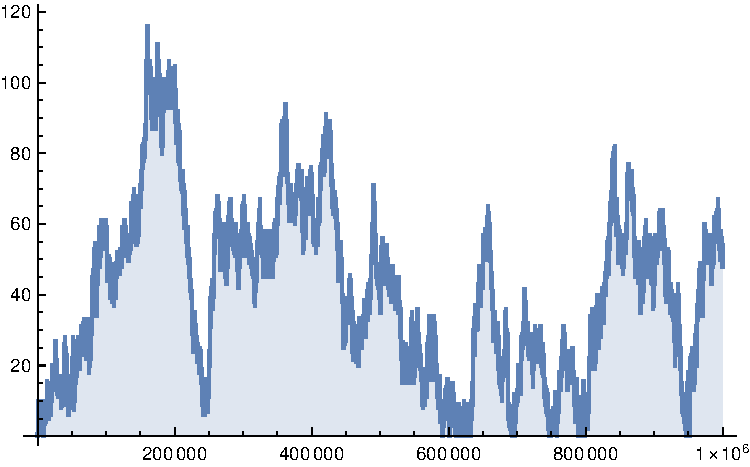
\includegraphics[width=0.8\textwidth]{abbildungen/1_Phone/Arrival_100_Serve_100_dur_1000000_Skip_0/QueueStepPlotAllFiltered.pdf}
	\caption{Warteschlangenlänge (gefiltert) , MeanAr = 100}
	\label{fig:QueueStepPlotAllFiltered100}
\end{figure}

\paragraph{Validierung der Simulation}
\begin{figure}[htpb]
	\centering
	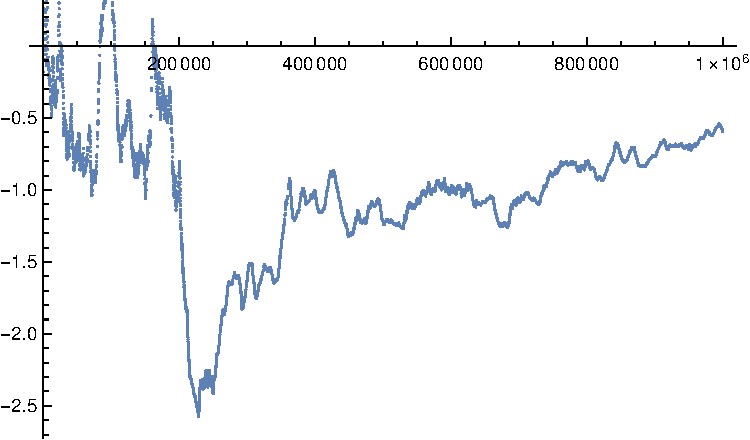
\includegraphics[width=0.8\textwidth]{abbildungen/1_Phone/Arrival_100_Serve_100_dur_1000000_Skip_0/LittleSystem.pdf}
	\caption{Darstellung der Differenz: $\lambda * Ws - Ls$ über die Simulationszeit (Little Theorem)}
	\label{fig:LittleSystem100}
\end{figure}
In Abbildung \ref{fig:LittleSystem100} ist der Verlauf der Gleichung \ref{eq:little} über die Simulationszeit aufgeführt. Im Vergleich zu den beiden Auswertungen mit Zwischenankunftszeiten von $1000s$ bzw. $400s$ wird deutlich, dass die Abweichung vom den geforderten Wert $0$ in dieser Abbildung erheblich größer ist.

Alle vier ermittelten Durchschnittswerte schwanken bis zum Ende der Simulation deutlich. Das in Abbildung \ref{fig:LittleSystem100} ersichtliche Ergebnis der Differenz zeigt, dass das System während der gesamten Simulationsdauer den für ein eingeschwungenes System erforderlichen Wert von $0$ nicht erreicht. Aufgrund der großen Abweichung kann davon ausgegangen werden, dass der Steady State (eingeschwungene Zustand) in dieser Simulation nicht erreicht wurde.

Das beschriebene Verhalten des implementierten Modells stimmt somit mit der Theorie überein, welche besagt, dass wenn die durchschnittliche Zwischenankunftszeit gleich der durchschnittlichen Bediendauer ist, das System nie einschwingen kann. Ein Beweis, dass das System auch bei einer längeren Simulationsdauer nicht einschwingen würde, kann nicht erbracht werden.

\subsubsection{Vergleich der Telefonauslastungen}
Bisher wurden die durschnittlichen Verweildauern betrachtet. Die Auslastung des Telefons wurde dabei unberücksichtigt. Die durchschnittliche Auslastung des telefons berechnet sich mit der Formel:
$$
Auslastung(t) = \frac{\sum Telefonierdauer}{t}
$$
Eine Auslastung von 1 bedeutet, dass das Telefon zu 100 \% ausgelastet ist. In Abbildung \ref{fig:1_Phone_Workload_Vergleich} werden die Auslastungen über der Zeit für verschiedene Ankunftsraten dargestellt. Es fällt auf, dass bei Ankunftszeiten von 1500 s bis 800 s nur wenig Unterschied besteht. Das Telefon ist in allen drei Fällen ca. 15 \% ausgelastet. Bei einer Ankunftszeit von 400 s gibt es einen deutlichen Anstieg in der Auslastung auf über 20 \%. Das Telefon ist zu 100 \% ausgelastet bei einer durchschnittlichen Zwischenankunftszeit von 100 s. Da die durchschnittliche Telefonierzeit ebenfalls 100 s beträgt, ist dieses Ergebnis zu erwarten. Es ist zu bemerken, dass die durchschnittliche Telefonauslastung und die Zwischenankunftszeiten keinen linearen Zusammenhang haben. Ein exponentieller Zusammenhang kann aufgrund der fünf Simulationen vermutet, jedoch nicht eindeutig gezeigt werden.
\begin{figure}[htpb]
	\centering
	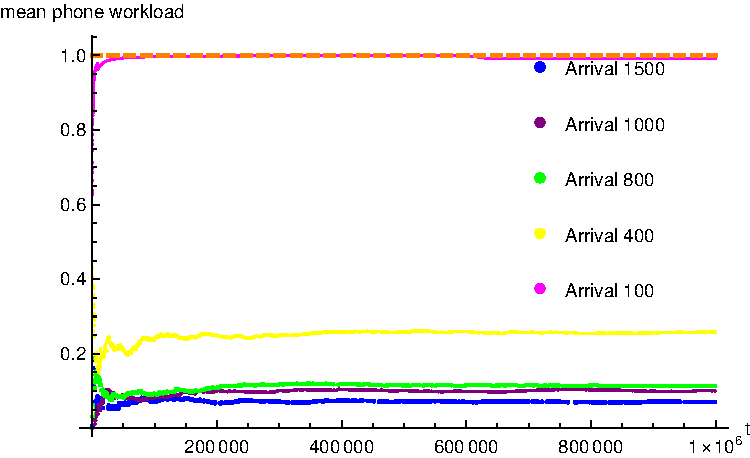
\includegraphics[width=0.8\textwidth]{abbildungen/1_Phone/Auslastung_Vegleich/MeanPhoneWorkload.pdf}
	\caption{Darstellung der Telefonauslastung für verschiedene Ankunftszeiten}
	\label{fig:1_Phone_Workload_Vergleich}
\end{figure}

Für ein aussagekräftigeres Ergebnis wurde die Siulation erneut mit einer längeren Simulationsdauer durchgeführt. Die Ergebnisse sind im folgenden Abschnitt beschrieben.

\subsubsection{Erhöhung der Simulationsdauer}

Die bisherigen Ergebnisse sind bei einer Simulationsdauer von $10^6 \ s$ entstanden. Bei einer Zwischenankunftszeit von 100 s zeigt sich eine Tendenz zu einer immer weiter ansteigenden Warteschlangenlänge. Um dies besser zu verdeutlichen wird die Simulationsdauer auf $10^7 s$ erhöht. Die Abbildung \ref{fig:QueueStepPlotAll100_duration_10000000} zeigt die Warteschlangenentwicklung über die gesamte Zeit. Es wird deutlich, dass die Warteschlangenlänge sehr schwankt. Aus den Abbildungen \ref{fig:meanQueueSize100_duration_10000000} und \ref{fig:meanSystemSize100_duration_10000000} ist für die durchschnittliche Warteschlangenlänge ein klarer Trend nach oben zu erkennen. Auch bei der Betrachtung der Verweildauern im System und in der Warteschlange, wie in Abbildungen \ref{fig:meanQueueTime100_duration_10000000} und \ref{fig:meanSystemTime100_duration_10000000} zu sehen ist, zeigt sich eine Aufwärtsbewegung. \\
Es ist deutlich zu erkennen, dass sich die Werte keiner Parallelen zur Zeitachse annähern. Das System erreicht während der gesamten Simulationsdauer keinen stabilen zustand. Bei einer weiteren Erhöhung der Simulationsdauer ist davon auszugehen, dass Werte noch weiter ansteigen werden.

\begin{figure}[htpb]
	\centering
	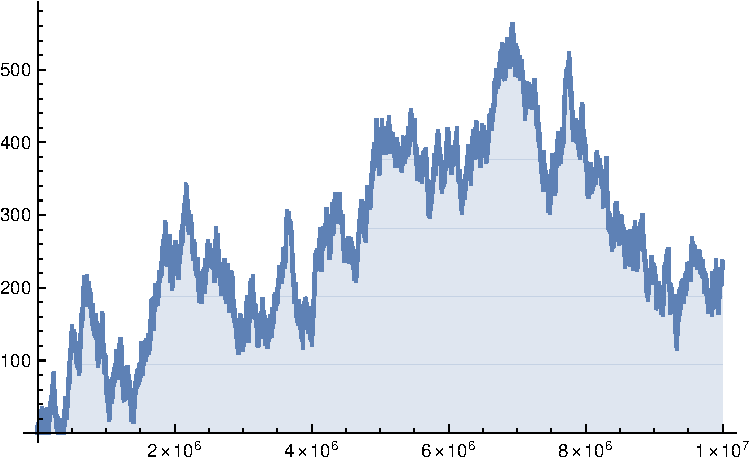
\includegraphics[width=0.8\textwidth]{abbildungen/1_Phone/Arrival_100_Serve_100_dur_10000000_Skip_0/QueueStepPlotAllFiltered.pdf}
	\caption{Warteschlangenlänge (gefiltert) , MeanAr = 100, Dauer = $10^7 \ s$}
	\label{fig:QueueStepPlotAll100_duration_10000000}
\end{figure}


\begin{figure}[htpb]
	\centering
	\includegraphics[width=0.8\textwidth]{abbildungen/1_Phone/Arrival_100_Serve_100_dur_10000000_Skip_0/MeanSystemSize.pdf}
	\caption{Durchschnittliche Anzahl an Kunden im System, MeanAr = $100s$, Dauer = $10^7 \ s$}
	\label{fig:meanSystemSize100_duration_10000000}
\end{figure}


\begin{figure}[htpb]
	\centering
	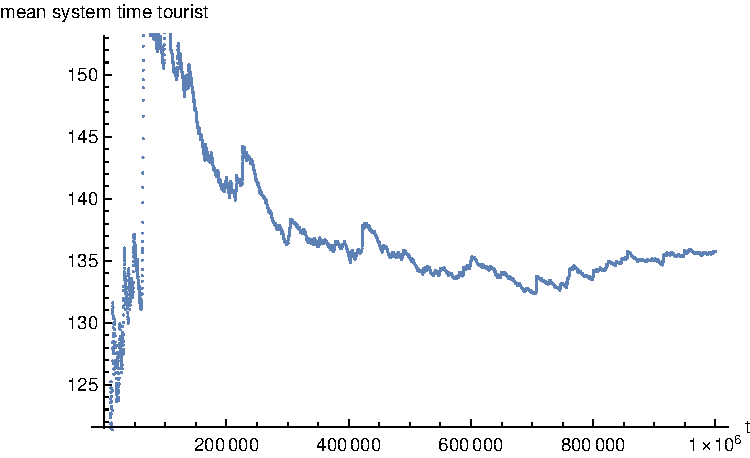
\includegraphics[width=0.8\textwidth]{abbildungen/1_Phone/Arrival_100_Serve_100_dur_10000000_Skip_0/MeanSystemTime.pdf}
	\caption{Durchschnittliche Verweildauer der Kunden im System, MeanAr = 100, Dauer = $10^7 \ s$}
	\label{fig:meanSystemTime100_duration_10000000}
\end{figure}



\begin{figure}[htpb]
	\centering
	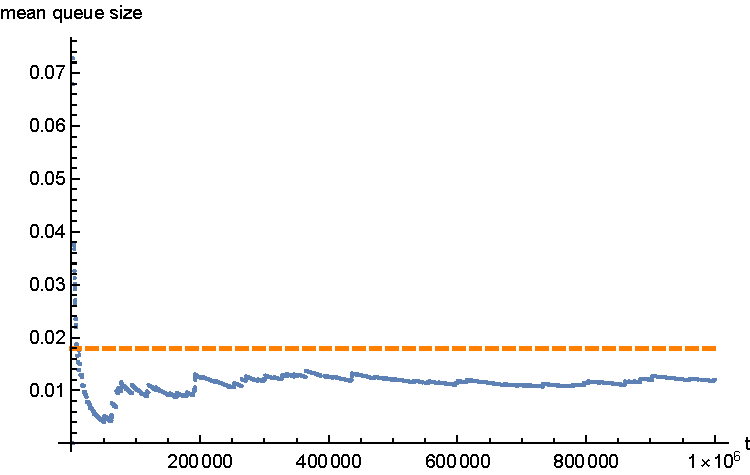
\includegraphics[width=0.8\textwidth]{abbildungen/1_Phone/Arrival_100_Serve_100_dur_10000000_Skip_0/MeanQueueSize.pdf}
	\caption{Durchschnittliche Warteschlangenlänge, MeanAr = 100, Dauer = $10^7 \ s$}
	\label{fig:meanQueueSize100_duration_10000000}
\end{figure}


\begin{figure}[htpb]
	\centering
	\includegraphics[width=0.8\textwidth]{abbildungen/1_Phone/Arrival_100_Serve_100_dur_10000000_Skip_0/MeanQueueTime.pdf}
	\caption{Durchschnittliche Verweildauer in der Warteschlange , MeanAr = 100, Dauer = $10^7 \ s$}
	\label{fig:meanQueueTime100_duration_10000000}
\end{figure}

Abbildung \ref{fig:LittleSystem100_duration_10000000} zeigt die Gleichung des Little Theorems für die Simulation mit erhöhter Simulationsdauer. Auch bei längerer Simulationsdauer wird der Wert von $0$ nicht erreicht. Die Abweichung wird mit steigender Simulationsdauer größer. Das System schwingt somit auch bei einer längeren Simulationsdauer nicht ein, was bei dieser Konstellation von durchschnittlicher Zwischwnankunftszeit und durchschnittlicher Telefonierdauer plausibel und gefordert ist.

\begin{figure}[htpb]
	\centering
	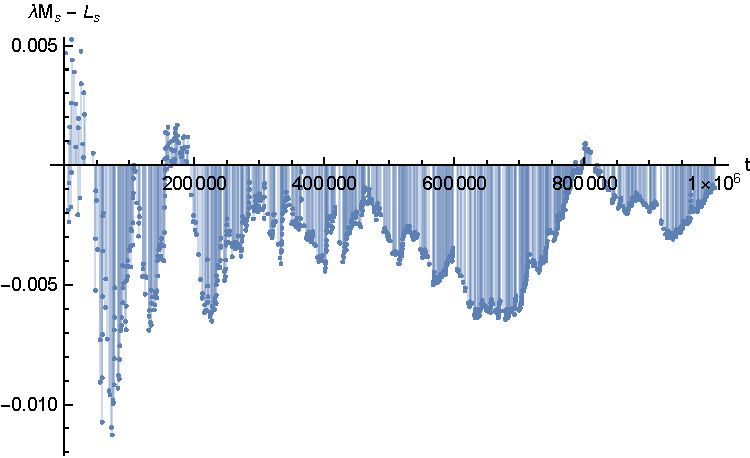
\includegraphics[width=0.8\textwidth]{abbildungen/1_Phone/Arrival_100_Serve_100_dur_10000000_Skip_0/LittleSystem.pdf}
	\caption{Darstellung der Differenz: $\lambda * Ws - Ls$ über die Simulationszeit (Little Theorem für die erhöhte Simulationsdauer)}
	\label{fig:LittleSystem100_duration_10000000}
\end{figure}

\subsection{Modell \glqq Bevorzugung der Einheimischen (VIP)\grqq}
Im zweiten Betriebsmodus werden die ankommenden Kunden unterschieden, ob es sich um Touristen, oder Einheimische (VIP) handelt. Befindet sich ein Einheimischer in der Warteschlange, wird dieser bevorzugt. Wie im Betriebsmodus 1 werden auch hier drei verschiedene mittleren Zwischenankunftszeiten betrachtet.

\subsubsection{Annahme}
Es wird angenommen, dass die im Abschnitt \ref{FormenlnMM1} aufgeführten Formeln für den Betriebsmodus 1 auch für diesen Betriebsmodus gelten. Da sich im Shop weiterhin nur ein Telefon befindet, ist es für die Berechnung der Durchschnittswerte für das System (durchschnittliche Anzahl an Kunden im System, durchschnittliche Warteschlangenlänge, durchschnittliche Zeit im System, durchschnittliche Zeit in der Warteschlange) irrelevant, ob bestimmte Kunden bevorzugt werden. Beispielsweise die durchschnittliche Zeit in der Warteschlange, welche bei den VIP durch die Bevorzugung geringer ist, ist bei den Touristen dementsprechend höher, sodass sie insgesamt gleich der Zeit im Betriebsmodus 1 ist.
\subsubsection{Durchschnittliche Ankunftszeit der Clients: 1000}
\paragraph{Theoretische Erwartungswerte laut M/M/1 Warteschlangenmodell}
\\
Bei einer durchschnittlichen Zwischenankunftszeit von $1000s$ ($\lambda=\frac{1}{1000}$, $\mu=\frac{1}{100}$)ergeben sich, basierend auf den in Abschnitt \ref{Formeln} aufgeführten Formeln, folgende Erwartungswerte:
\begin{equation}
Ls=0,111111
\end{equation}
\begin{equation}
Lq=0,0111111
\end{equation}
\begin{equation}
Ws=111,111
\end{equation}
\begin{equation}
Wq=11,1111
\end{equation}
\paragraph{Verwendung der implementierten Java-Simulation, Berechnung in Java}
\label{JavaVIPPhone1000}
\\
\begin{figure}[htpb]
	\centering
	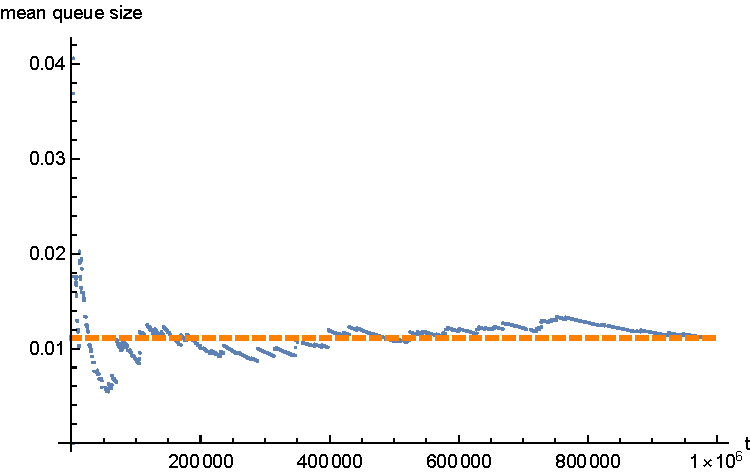
\includegraphics[width=0.8\textwidth]{abbildungen/1_Phone_VIP/Arrival_1000_Serve_100_dur_1000000_Skip_0/MeanQueueSizeAll.pdf}
	\caption{Durchschnittliche Warteschlangenlänge, MeanAr = 1000}
	\label{fig:MQSVIP1000ALL}
\end{figure}

\begin{figure}[htpb]
	\centering
	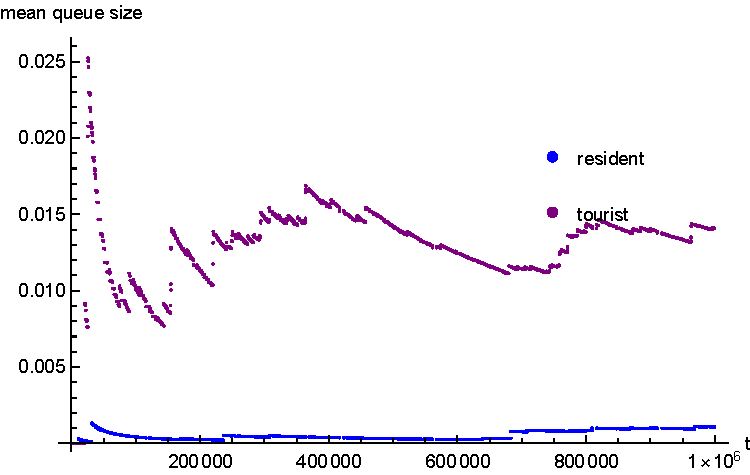
\includegraphics[width=0.8\textwidth]{abbildungen/1_Phone_VIP/Arrival_1000_Serve_100_dur_1000000_Skip_0/MeanQueueSizeTouristAndResident.pdf}
	\caption{Durchschnittliche Warteschlangenlängen von Touristen und VIP, MeanAr = 1000}
	\label{fig:MQSVIP1000VGL}
\end{figure}

Abbildung \ref{fig:MQSVIP1000ALL} zeigt die durchschnittliche Warteschlangenlänge. Im Vergleich dazu zeigt Abbildung \ref{fig:MQSVIP1000VGL} die Zusammensetzung der Warteschlangenlänge aus den zwei unterschiedenen Gruppen. Es wird deutlich, dass die Wartezeit der Touristen deutlich länger ist als die der Einheimischen, was aufgrund der Bevorzugung plausibel ist. Die durchschnittliche Warteschlangenlänge insgesamt liegt gegen Ende der Simulation um ca. $0,004$ über dem erwarteten Wert von $0.111111$ (gelbe Linie). Doch neben der Bevorzugung spielt auch der Anteil der Einheimischen an der insgesamten Kundenanzahl (lediglich $0,1$) eine Rolle. Es kommen somit deutlich mehr Touristen in den Telefonshop als Einheimische.

\begin{figure}[htpb]
	\centering
	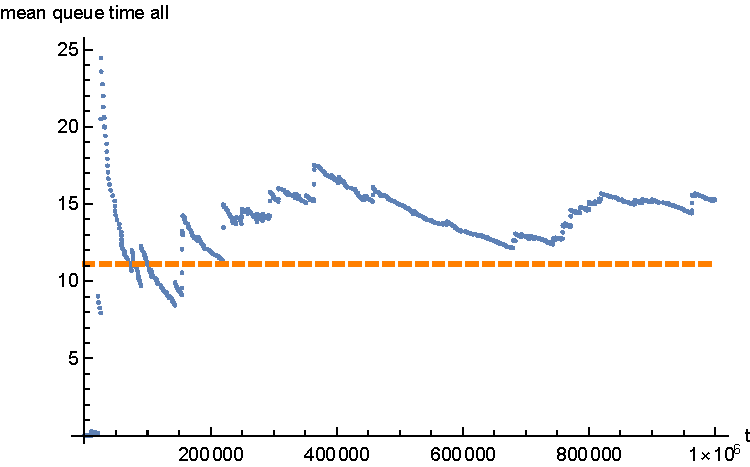
\includegraphics[width=0.8\textwidth]{abbildungen/1_Phone_VIP/Arrival_1000_Serve_100_dur_1000000_Skip_0/MeanQueueTimeAll.pdf}
	\caption{Durchschnittliche Verweildauer in der Warteschlange, MeanAr = 1000}
	\label{fig:MQTVIP1000ALL}
\end{figure}

\begin{figure}[htpb]
	\centering
	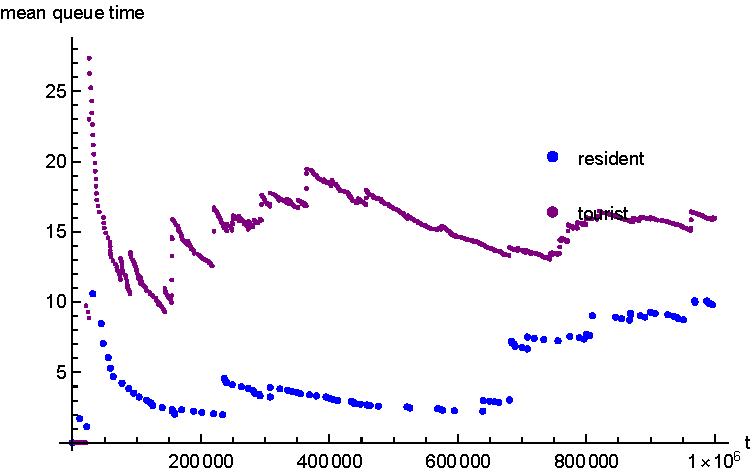
\includegraphics[width=0.8\textwidth]{abbildungen/1_Phone_VIP/Arrival_1000_Serve_100_dur_1000000_Skip_0/MeanQueueTimeTouristAndResident.pdf}
	\caption{Durchschnittliche Verweildauer der Touristen und Einheimische in der Warteschlange , MeanAr = $1000s$}
	\label{fig:MQTVIP1000VGL}
\end{figure}

In der Abbildung \ref{fig:MQTVIP1000ALL} sieht man die durchschnittliche Wartezeit aller Kunden insgesamt. Im Vergleich dazu wird in der Abbildung \ref{fig:MQTVIP1000VGL} zwischen Touristen und Einheimischen unterschieden. Durch die Bevorzugung ist auch hier der Wert der Einheimischen deutlich geringer als der der Touristen. Auffallend ist ebenfalls, dass bei Simulationsdauer von ca. $680000s$ die Anzahl der wartenden Einheimischen leicht ansteigt. In etwa zur gleichen Zeit steigt die durchschnittliche Wartezeit der Einheimischen ebenfalls an. Da jedoch durch die geringe Auslastung des Telefons die insgesamte Wartezeit beider Gruppen sehr gering ist, scheint die durchschnittliche Wartezeit der Einheimischen zu diesem Zeitpunkt deutlich drastischer anzusteigen als die Anzahl. Dies liegt jedoch lediglich an der feineren Skalierung und wäre auch nicht plausibel.

\begin{figure}[htpb]
	\centering
	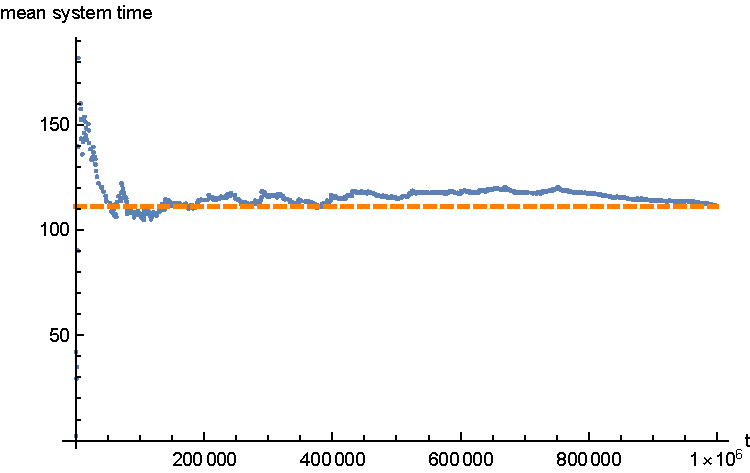
\includegraphics[width=0.8\textwidth]{abbildungen/1_Phone_VIP/Arrival_1000_Serve_100_dur_1000000_Skip_0/MeanSystemTimeAll.pdf}
	\caption{Durchschnittliche Verweildauer der Kunden im System, MeanAr = $1000s$}
	\label{fig:MSTVIP1000ALL}
\end{figure}

\begin{figure}[htpb]
	\centering
	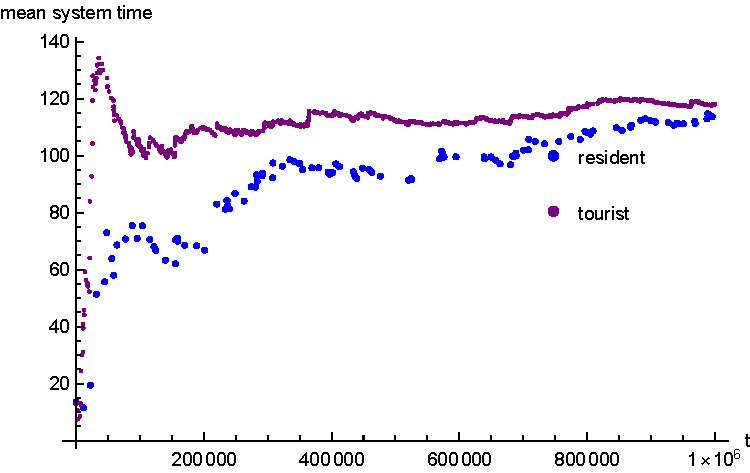
\includegraphics[width=0.8\textwidth]{abbildungen/1_Phone_VIP/Arrival_1000_Serve_100_dur_1000000_Skip_0/MeanSystemTimeTouristAndResident.pdf}
	\caption{Durchschnittliche Verweildauer der Einheimischen und Touristen im System, MeanAr = $1000s$}
	\label{fig:MSTVIP1000VGL}
\end{figure}

Abbildung \ref{fig:MSTVIP1000ALL} zeigt die durchschnittliche Verweildauer aller Kunden im System insgesamt. Im Vergleich dazu zeigt Abbildung \ref{fig:MSTVIP1000VGL} die Zusammensetzung aus den zwei unterschiedenen Gruppen. Die durchschnittliche Verweildauer insgesamt liegt wiederum im Bereich des Erwartungswertes (Abweichung ca. $10s$). Interessant ist hingegen die Aufteilung zwischen den Touristen und Einheimischen. Obwohl die Werte für die Verweildauer in der Warteschlange und auch für die Warteschlangenlänge bei den Einheimischen deutlich niedriger waren, als bei den Touristen, liegen die Werte in diesem Fall, vor allem gegen Ende der Simulationszeit, sehr nah beieinander. Die Ursache hierfür liegt in der geringen Auslastung des Telefons. Durch die durchschnittliche Telefonierdauer von $100s$ liegt die durchschnittliche Verweildauer im System ohne Wartezeit ebenfalls bei $100s$. Da auch die bevorzugten Einheimischen warten müssen, bis ein belegtes Telefon wieder frei ist, bevor sie telefonieren können, liegt der Wert hier entwas über $100s$. Da jedoch das Telefon nur gering ausgelastet ist, müssen auch die Touristen durchschnittlich nur eine sehr kurze Zeit warten und haben daher auch nur eine durchschnittliche Verweildauer im System von ca. $118s$.

\begin{figure}[htpb]
	\centering
	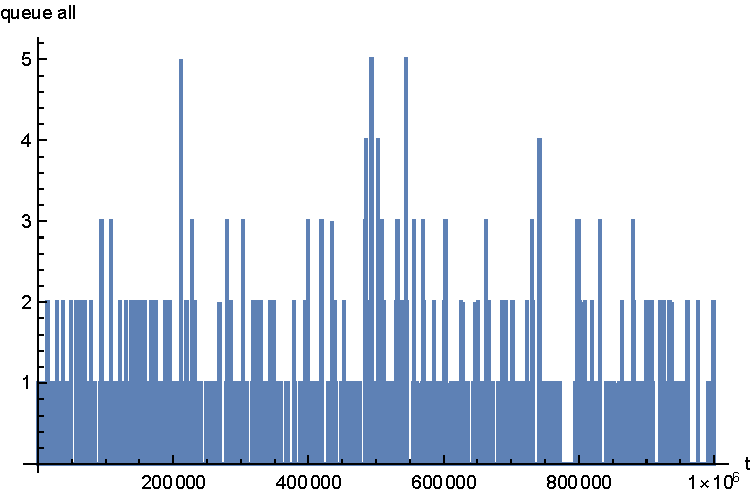
\includegraphics[width=0.8\textwidth]{abbildungen/1_Phone_VIP/Arrival_400_Serve_100_dur_1000000_Skip_0/QueueStepPlotAllFiltered.pdf}
	\caption{Warteschlangenlänge insgesamt (gefiltert), MeanAr = $400s$}
	\label{fig:QSPALL400}
\end{figure}

\begin{figure}[htpb]
	\centering
	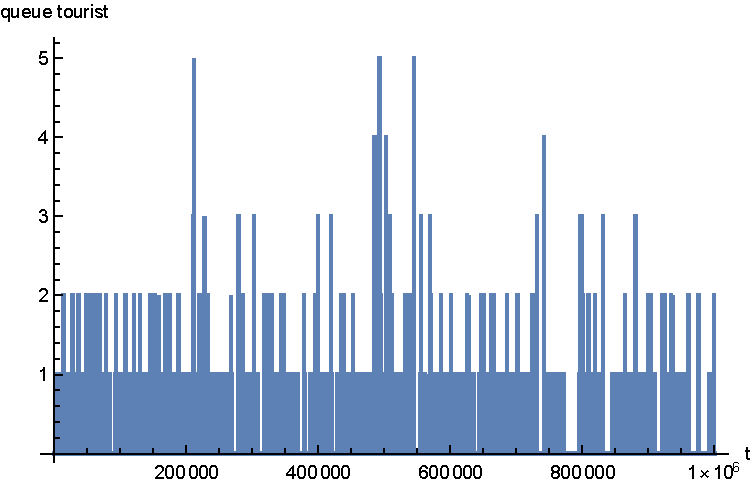
\includegraphics[width=0.8\textwidth]{abbildungen/1_Phone_VIP/Arrival_400_Serve_100_dur_1000000_Skip_0/QueueStepPlotTouristFiltered.pdf}
	\caption{Warteschlangenlänge der Touristen (gefiltert), MeanAr = $400s$}
	\label{fig:QSPTOURI400}
\end{figure}

\begin{figure}[htpb]
	\centering
	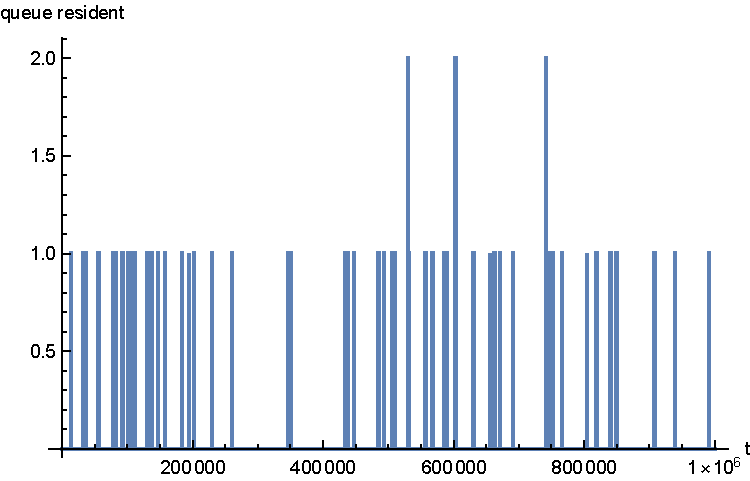
\includegraphics[width=0.8\textwidth]{abbildungen/1_Phone_VIP/Arrival_400_Serve_100_dur_1000000_Skip_0/QueueStepPlotResidentFiltered.pdf}
	\caption{Warteschlangenlänge der Einheimischen (gefiltert), MeanAr = $400s$}
	\label{fig:QSPVIP400}
\end{figure}

Die Abbildungen \ref{fig:QSPALL1000}, \ref{fig:QSPTOURI1000} und \ref{fig:QSPVIP1000} zeigen die absoluten Warteschlangenlängen zu den unterschiedlichen Systemzeiten. Über die gesamte Simulationszeit ist die maximal auftretende Warteschlangenlänge lediglich $5$. Es warten jedoch, wie Abbildung \ref{fig:QSPVIP1000} zeigt zu keinem Zeitpunkt zwei Einheimische gleichzeitig. Dies belegt die geringe durchschnittliche Verweildauer der Einheimischen im System und in der Warteschlange.

\paragraph{Validierung der Simulation}
\\
\begin{figure}[htpb]
	\centering
	\includegraphics[width=0.8\textwidth]{abbildungen/1_Phone_VIP/Arrival_1000_Serve_100_dur_1000000_Skip_0/LittleSystem.pdf}
	\caption{Darstellung der Differenz: $\lambda * Ws - Ls$ über die Simulationszeit (Little Theorem)}
	\label{fig:LittleSystemVIP1000}
\end{figure}

In Abbildung \ref{fig:LittleSystemVIP1000} ist der Verlauf der Gleichung \ref{eq:little} über die Simulationszeit aufgeführt. Ab einer Simulationsdauer von ca. $250000s$ schwankt der Wert nur noch um einen Wert von ca. $0,005$. Gegen Ende der Simulation steigt der Wert in Richtung Nulllinie an und liegt am Ende bei ca. $-0,001$. Diese sehr geringe Abweichung zeigt, dass das System mit großer Wahrscheinlichkeit eingeschwungen ist. Die Abweichung von $0,001$ ist sehr gering und auf kleinere Rundungsfehler bei der Berechnung zurückzuführen.




\subsubsection{Durchschnittliche Ankunftszeit der Clients: 400}
\paragraph{Theoretische Erwartungswerte laut M/M/1 Warteschlangenmodell}
\\
Bei einer durchschnittlichen Zwischenankunftszeit von $400s$ ($\lambda=\frac{1}{400}$, $\mu=\frac{1}{100}$)ergeben sich, basierend auf den in Abschnitt \ref{Formeln} aufgeführten Formeln, folgende Erwartungswerte:
\begin{equation}
Ls=0,333333
\end{equation}
\begin{equation}
Lq=0,0833333
\end{equation}
\begin{equation}
Ws=133,333
\end{equation}
\begin{equation}
Wq=33,3333
\end{equation}

\paragraph{Verwendung der implementierten Java-Simulation, Berechnung in Java}
\label{JavaVIPPhone400}
\\
\begin{figure}[htpb]
	\centering
	\includegraphics[width=0.8\textwidth]{abbildungen/1_Phone_VIP/Arrival_400_Serve_100_dur_1000000_Skip_0/MeanQueueSizeAll.pdf}
	\caption{Durchschnittliche Warteschlangenlänge, MeanAr = 400}
	\label{fig:MQSVIP400ALL}
\end{figure}

\begin{figure}[htpb]
	\centering
	\includegraphics[width=0.8\textwidth]{abbildungen/1_Phone_VIP/Arrival_400_Serve_100_dur_1000000_Skip_0/MeanQueueSizeTouristAndResident.pdf}
	\caption{Durchschnittliche Warteschlangenlängen von Touristen und VIP, MeanAr = $400s$}
	\label{fig:MQSVIP400VGL}
\end{figure}

Abbildung \ref{fig:MQSVIP400ALL} zeigt die durchschnittliche Warteschlangenlänge. Im Vergleich dazu zeigt Abbildung \ref{fig:MQSVIP400VGL} die Zusammensetzung der Warteschlangenlänge aus den zwei unterschiedenen Gruppen. Wie bei einer durchschnittlichen Zwischenankunftszeit von $1000s$, fällt auch hier auf, dass sich deutlich weniger Einheimische in der Warteschlange befinden als Touristen. Beide Werte sind jedoch höher als bei einer durchschnittlichen Zwischenankunftszeit von $1000s$, was aufgrund der höheren Auslastung des Telefons plausibel ist. Der Wert von beiden Gruppen zusammengenommen schwankt um den erwarteten Wert von $0,0833333$ und nähert sich diesem gegen Ende der Simulation immer weiter an. Am Ende liegt eine Abweichung von ca. $0,007$ vor.

\begin{figure}[htpb]
	\centering
	\includegraphics[width=0.8\textwidth]{abbildungen/1_Phone_VIP/Arrival_400_Serve_100_dur_1000000_Skip_0/MeanQueueTimeAll.pdf}
	\caption{Durchschnittliche Verweildauer in der Warteschlange, MeanAr = $400s$}
	\label{fig:MQTVIP400ALL}
\end{figure}

\begin{figure}[htpb]
	\centering
	\includegraphics[width=0.8\textwidth]{abbildungen/1_Phone_VIP/Arrival_400_Serve_100_dur_1000000_Skip_0/MeanQueueTimeTouristAndResident.pdf}
	\caption{Durchschnittliche Verweildauer der Touristen und Einheimische in der Warteschlange , MeanAr = $400s$}
	\label{fig:MQTVIP400VGL}
\end{figure}

In der Abbildung \ref{fig:MQTVIP400ALL} sieht man die durchschnittliche Wartezeit aller Kunden insgesamt. Im Vergleich dazu wird in der Abbildung \ref{fig:MQTVIP400VGL} zwischen Touristen und Einheimischen unterschieden. Ab einer Simulationsdauer von ca. $300000s$ ist, aufgrund der Bevorzugung, auch hier der Wert der Einheimischen deutlich geringer als der der Touristen. Auffallend ist, dass der Wert der Einheimischen zu Beginn der Simulation kurzzeitig höher ist als der der Touristen. Hintergrund dürfte hierbei ein nicht eingeschwungenes System sein, infolge dessen einzelne Kunden noch eine große Veränderung des durschnittswertes bewirken. Gegen Ende der Simulation näher sich der errechnete Wert immer weiter dem Erwartungswert von $33,3333$ an. Am Ende der Simulation ist eine Abweichung von ca. $1,5$ anzumerken.

\begin{figure}[htpb]
	\centering
	\includegraphics[width=0.8\textwidth]{abbildungen/1_Phone_VIP/Arrival_400_Serve_100_dur_1000000_Skip_0/MeanSystemTimeAll.pdf}
	\caption{Durchschnittliche Verweildauer der Kunden im System, MeanAr = $400s$}
	\label{fig:MSTVIP400ALL}
\end{figure}

\begin{figure}[htpb]
	\centering
	\includegraphics[width=0.8\textwidth]{abbildungen/1_Phone_VIP/Arrival_400_Serve_100_dur_1000000_Skip_0/MeanSystemTimeTouristAndResident.pdf}
	\caption{Durchschnittliche Verweildauer der Einheimischen und Touristen im System, MeanAr = $400s$}
	\label{fig:MSTVIP400VGL}
\end{figure}

Abbildung \ref{fig:MSTVIP1000ALL} zeigt die durchschnittliche Verweildauer aller Kunden im System insgesamt. Im Vergleich dazu zeigt Abbildung \ref{fig:MSTVIP1000VGL} die Zusammensetzung aus den zwei unterschiedenen Gruppen. Wiederum zeigt sich, dass der Wert der Einheimischen zu Beginn der Simulation kurzzeitig höher ist als der der Touristen. Dies stimmt mit Abbildung \ref{fig:MQTVIP400VGL} überein, spricht jedoch für ein (bis zu diesem Zeitpunkt) nicht eingeschwungenes System. Der Wert der Einheimischen liegt ab einer Simulationsdauer von $400000s$ bei ca. $125s$. Dies setzt sich aus einer durchschnittlichen Telefonierdauer von $100s$ und der durchschnittlichen Verweildauer ca. $25s$ zusammen (siehe Abbildung \ref{fig:MQTVIP400VGL})  und ist somit plausibel. Die durchschnittliche Verweildauer beider Gruppen zusammen nähert sich ab einer Simulationsdauer von ca. $400000s$ dem erwarteten Wert von $133,333$ immer weiter an. Gegen Ende der Simulation ist eine Abweichung von ca. $3s$ festzustellen.

\begin{figure}[htpb]
	\centering
	\includegraphics[width=0.8\textwidth]{abbildungen/1_Phone_VIP/Arrival_1000_Serve_100_dur_1000000_Skip_0/QueueStepPlotAllFiltered.pdf}
	\caption{Warteschlangenlänge insgesamt (gefiltert), MeanAr = $1000s$}
	\label{fig:QSPALL1000}
\end{figure}

\begin{figure}[htpb]
	\centering
	\includegraphics[width=0.8\textwidth]{abbildungen/1_Phone_VIP/Arrival_1000_Serve_100_dur_1000000_Skip_0/QueueStepPlotTouristFiltered.pdf}
	\caption{Warteschlangenlänge der Touristen (gefiltert), MeanAr = $1000s$}
	\label{fig:QSPTOURI1000}
\end{figure}

\begin{figure}[htpb]
	\centering
	\includegraphics[width=0.8\textwidth]{abbildungen/1_Phone_VIP/Arrival_1000_Serve_100_dur_1000000_Skip_0/QueueStepPlotResidentFiltered.pdf}
	\caption{Warteschlangenlänge der Einheimischen (gefiltert), MeanAr = $1000s$}
	\label{fig:QSPVIP1000}
\end{figure}


\paragraph{Validierung der Simulation}
\\
\begin{figure}[htpb]
	\centering
	\includegraphics[width=0.8\textwidth]{abbildungen/1_Phone_VIP/Arrival_400_Serve_100_dur_1000000_Skip_0/LittleSystem.pdf}
	\caption{Darstellung der Differenz: $\lambda * Ws - Ls$ über die Simulationszeit (Little Theorem)}
	\label{fig:LittleSystemVIP400}
\end{figure}

In Abbildung \ref{fig:LittleSystemVIP400} ist der Verlauf der Gleichung \ref{eq:little} über die Simulationszeit aufgeführt. Ab einer Simulationsdauer von ca. $450000s$ schwankt der Wert nur noch um einen Wert von ca. $0,01$. Gegen Ende der Simulation schwankt der Wert um die Nulllinie und weicht am Ende nur noch um ca. $0,002$ ab. Diese sehr geringe Abweichung zeigt, dass das System mit großer Wahrscheinlichkeit eingeschwungen ist. Die Abweichung von $0,002$ ist sehr gering und auf kleinere Rundungsfehler bei der Berechnung zurückzuführen.

\subsubsection{Durchschnittliche Ankunftszeit der Clients: 100}
Es wird eine Simulation durchgeführt, mit einer durschnittlichen Zwischenankunftszeit von 100 s. Dabei wird zwischen den Einheimischen und den Touristen unterschieden. Die Einheimischen stellen 10 \% der Besucher dar. Da die Einheimischen bevorzugt behandelt werden, ist anzunehmen, dass die durchschnittlichen Verweildauern im System und in der Warteschlange niedriger sind. Wie bereits aus vorherigen Simulationen hervorgegangen ist, laufen die Verweildauern und die Warteschlangenlänge gegen Unendlich. Es ist zu untersuchen, wie sich die Verweildauern für Einheimische verhalten. Die Abbildungen \ref{fig:1_Phone_VIP_100_MeanQueueSize_Tourist} und \ref{fig:1_Phone_VIP_100_MeanQueueSize_Resident} zeigen, dass, sich die durchschnittliche Warteschlangenlänge von Touristen und Einheimischen deutlich unterscheiden. Die durschnittliche Warteschlangenlänge der Einheimischen geht ungefähr gegen 0.1, während die der Touristen gegen unendlich steigt. Die Abbildung \ref{fig:1_Phone_VIP_100_MeanQueueSize_All} verdeutlicht nochmals diesen Zusammenhang. \\
Ähnlich sieht es auch bei den Verweildauern aus. Die durchschnittliche Wartezeit der Einheimischen beträgt ungefähr 110 s, während die Wartezeit der Touristen gegen unendlich läuft. Dieser Zusammenhang ist in den Abbildungen \ref{fig:1_Phone_VIP_100_MeanQueueTime_Tourist} und \ref{fig:1_Phone_VIP_100_MeanQueueTime_Resident}. Die Abbildung \ref{fig:1_Phone_VIP_100_MeanQueueTime_All} Vergleicht die Wartezeiten miteinander. Es ist logisch zu erklären, dass sich die Wartezeit der Einheimischen auf den wert nahe an 100 s einpendelt. Einheimische werden nur bevorzugt, wenn das Telefon frei ist. Ist das Telefon besetzt, müssen auch die Einheimischen warten. Da die durchschnittliche Telefonierdauer 100 s beträgt, müssen die Einheimischen mindestens diese Zeit abwarten. Der Wert ist etwas größer als 100, da die Einheimischen auch warten müssen, wenn sich weitere Einheimische in der Warteschlange befinden.\\
Interessant ist die Tatsache, dass die Wartezeit der Einheimischen bis ca. 100.000 s Simulationsdauer nahezu 0 beträgt und danach Sprunghaft ansteigt. Die ist damit zu erklären, dass ab dieser Zeit die Warteschlange sprunghaft ansteigt wie in Abbildung \ref{fig:1_Phone_VIP_100_QueuePlot_All} zu sehen ist. Auch die Betrachtung der Telefonauslastung bestätigt diese Vermutung. Die Abbildung \ref{fig:1_Phone_VIP_100_WorkLoad} zeigt, wie sich die Auslastung zunächst verringert und nach 100.000 s Simulationsdauer ansteigt. \\
Die Abbildung \ref{fig:1_Phone_VIP_100_MeanSystemTime_Resident} zeigt, dass sich die durchschnittliche Systemzeit der Einheimischen bei ungefähr 200 einpendelt. Das ist logisch, da sich die Systemzeit aus der Wartezeit und der Telefonierzeit zusammensetzt. Muss ein Einheimischer im Schnitt 100 s warten und 100 s telefonieren, dann verbleibt er im Schnitt 200 s im System.\\
Da Einheimische bevorzugt behandelt werden und einen Anteil von 10 \% der Besucher ausmachen, kommen die Einheimischen durschnittlich alle 1000 s an. Dies könnte zum Irrtum führen, dass die Verweildauern der Einheimischen ähnlich zu betrachten sind, als würde man die eine Simulation ohne Bevorzugung für eine Ankunftszeit von 1000 s durchführen. Die ist jedoch nicht richtig. Obwohl die Einheimischen bevorzugt werden, ist ihre Wartezeit direkt von der Telefonauslastung abhängig. Ist das Telefon voll Ausgelastet, müssen die Einheimischen im Schnitt 100 s warten. Also rund das zehnfache, als die Werte in Abbildung \ref{fig:meanQueueTime1000}. Anders würde das Ergebnis aussehen, wenn Touristen ihr Telefonat unterbrechen müssten, sobald ein Einheimischer die Warteschlange betritt.
\subsubsection{Eingeschwungener Zustand \ Littles Gesetz}
Die Abbildung \ref{fig:1_Phone_VIP_100_Little} zeigt den Verlauf der Gleichung \ref{eq:little}. Es ist deutlich zu erkennen, dass es noch große Schwankungen gibt und das System sich in einem nicht stabilen Zustand befindet. Es ist anzunehmen, dass bei einer durschnittlichen Zwischenankunftszeit die gleich der durchschnittlichen Telefonierdauer ist, sich das System nicht in einem stabilen Zustand befinden kann.

\begin{figure}[htpb]
	\centering
	\includegraphics[width=0.8\textwidth]{abbildungen/1_Phone_VIP/Arrival_100_Serve_100_dur_1000000_Skip_0/MeanQueueSizeTourist.pdf}
	\caption{Durchschnittliche Warteschlangenlänge der Touristen bei einer Zwischenankunftszeit von 100 s}
	\label{fig:1_Phone_VIP_100_MeanQueueSize_Tourist}
\end{figure}

\begin{figure}[htpb]
	\centering
	\includegraphics[width=0.8\textwidth]{abbildungen/1_Phone_VIP/Arrival_100_Serve_100_dur_1000000_Skip_0/MeanQueueSizeResident.pdf}
	\caption{Durchschnittliche Warteschlangenlänge der Einheimischen bei einer Zwischenankunftszeit von 100 s}
	\label{fig:1_Phone_VIP_100_MeanQueueSize_Resident}
\end{figure}

\begin{figure}[htpb]
	\centering
	\includegraphics[width=0.8\textwidth]{abbildungen/1_Phone_VIP/Arrival_100_Serve_100_dur_1000000_Skip_0/MeanQueueSizeTouristAndResident.pdf}
	\caption{Durchschnittliche Warteschlangenlänge der Einheimischen und Touristen bei einer Zwischenankunftszeit von 100 s}
	\label{fig:1_Phone_VIP_100_MeanQueueSize_All}
\end{figure}



\begin{figure}[htpb]
	\centering
	\includegraphics[width=0.8\textwidth]{abbildungen/1_Phone_VIP/Arrival_100_Serve_100_dur_1000000_Skip_0/MeanQueueTimeTourist.pdf}
	\caption{Durchschnittliche Wartezeit der Touristen bei einer Zwischenankunftszeit von 100 s}
	\label{fig:1_Phone_VIP_100_MeanQueueTime_Tourist}
\end{figure}

\begin{figure}[htpb]
	\centering
	\includegraphics[width=0.8\textwidth]{abbildungen/1_Phone_VIP/Arrival_100_Serve_100_dur_1000000_Skip_0/MeanQueueTimeResident.pdf}
	\caption{Durchschnittliche Wartezeit der Einheimischen bei einer Zwischenankunftszeit von 100 s}
	\label{fig:1_Phone_VIP_100_MeanQueueTime_Resident}
\end{figure}

\begin{figure}[htpb]
	\centering
	\includegraphics[width=0.8\textwidth]{abbildungen/1_Phone_VIP/Arrival_100_Serve_100_dur_1000000_Skip_0/MeanQueueTimeTouristAndResident.pdf}
	\caption{Durchschnittliche Wartezeit der Einheimischen und Touristen bei einer Zwischenankunftszeit von 100 s}
	\label{fig:1_Phone_VIP_100_MeanQueueTime_All}
\end{figure}


\begin{figure}[htpb]
	\centering
	\includegraphics[width=0.8\textwidth]{abbildungen/1_Phone_VIP/Arrival_100_Serve_100_dur_1000000_Skip_0/MeanSystemTimeResident.pdf}
	\caption{Durchschnittliche Systemzeit der Einheimischen bei einer Zwischenankunftszeit von 100 s}
	\label{fig:1_Phone_VIP_100_MeanSystemTime_Resident}
\end{figure}

\begin{figure}[htpb]
	\centering
	\includegraphics[width=0.8\textwidth]{abbildungen/1_Phone_VIP/Arrival_100_Serve_100_dur_1000000_Skip_0/QueueStepPlotAllFiltered.pdf}
	\caption{Warteschlange über den gesamten Simulationsverlauf bei einer Zwischenankunftszeit von 100 s}
	\label{fig:1_Phone_VIP_100_QueuePlot_All}
\end{figure}



\begin{figure}[htpb]
	\centering
	\includegraphics[width=0.8\textwidth]{abbildungen/1_Phone_VIP/Arrival_100_Serve_100_dur_1000000_Skip_0/MeanPhoneWorkload.pdf}
	\caption{Durchschnittliche Auslastung des Telefons bei einer Zwischenankunftszeit von 100 s}
	\label{fig:1_Phone_VIP_100_WorkLoad}
\end{figure}



\begin{figure}[htpb]
	\centering
	\includegraphics[width=0.8\textwidth]{abbildungen/1_Phone_VIP/Arrival_100_Serve_100_dur_1000000_Skip_0/LittleSystem.pdf}
	\caption{Darstellung der Differenz: $\lambda * Ws - Ls$ über die Simulationszeit (Little Theorem) bei einer Zwischenankunftszeit von 100 s}
	\label{fig:1_Phone_VIP_100_Little}
\end{figure}




\subsection{Modell \glqq Zusätzliches VIP Telefon\grqq}
Im dritten Betriebsmodus wird zu einem Telefon wie im Betriebsmodus 1 ein VIP Telefon (Telefon, welches Einheimische bevorzugt) hinzugefügt. Wie vorhin werden auch hier die drei verschiedenen mittleren Ankunftszeiten betrachtet. In diesem Szenario werden die Formeln für M/M/2 Warteschlangenmodelle verwendet.
\subsubsection{Formeln für M/M/2 Warteschlangenmodelle}
\label{Formeln2}
Für die theoretischen Größen und Zeiten des Systems bzw. der Warteschlange werden folgende Formeln genutzt [3]. Dabei steht P0 für die Wahrscheinlichkeit, dass sich keine Kunden im System befinden. Der Wert c steht für die Anzahl der Telefone. In diesem Betriebsmodus also c = $2$.
\begin{equation}
P0=(1+\rho+\rho^2/(2-\rho))^{-1}
\end{equation}
\begin{equation}
Ls=\rho + \frac{P0*\rho^{c+1}}{(c-\rho)!(c-\rho)^2}
\end{equation}
\begin{equation}
Lq=\frac{P0*\rho^{c+1}}{(c-1)!(c-\rho)^2}
\end{equation}
\begin{equation}
Wq=\frac{Lq}{\lambda}
\end{equation}
\begin{equation}
Ws=\frac{Ls}{\lambda}
\end{equation}
\subsubsection{Durchschnittliche Ankunftszeit der Clients: 1000}
\paragraph{Theoretische Erwartungswerte laut M/M/2 Warteschlangenmodell}
\\
Bei einer durchschnittlichen Zwischenankunftszeit von $1000s$ ($\lambda=\frac{1}{1000}$, $\mu=\frac{1}{100}$)ergeben sich, basierend auf den in Abschnitt \ref{Formeln2} aufgeführten Formeln, folgende Erwartungswerte:
\begin{equation}
Ls=0,100137
\end{equation}
\begin{equation}
Lq=0,000250627
\end{equation}
\begin{equation}
Ws=100,137
\end{equation}
\begin{equation}
Wq=0,250627
\end{equation}

\paragraph{Verwendung der implementierten Java-Simulation, Berechnung in Java}
\label{JavaTwoPhones1000}
\\
\begin{figure}[htpb]
	\centering
	\includegraphics[width=0.8\textwidth]{abbildungen/2_Phone_VIP/Arrival_1000_Serve_100_dur_1000000_Skip_0/MeanSystemSizeAll.pdf}
	\caption{Durchschnittliche Anzahl an Kunden im System, MeanAr = $1000s$}
	\label{fig:mean3SystemSize1000}
\end{figure}

Abbildung \ref{fig:mean3SystemSize1000} zeigt die durchschnittliche Anzahl an Kunden im System an. Ab einer Simulationszeit von ca $300000s$ liegt diese durchschnittlich bei $0.10$, steigt jedoch bis zum Ende der Simulation um ca. $0,01$. Der Erwartungswert von $0,100137$ wird auch hier durch die Simulation nicht exakt erreicht. Auch in dieser Berechnung muss von einem systematischen Fehler von ca. $0,01$ ausgegangen werden. Die geringe Abweichung lässt anzunehmen, dass die Systemgröße für dieses Szenario plausibel ist.

\begin{figure}[htpb]
	\centering
	\includegraphics[width=0.8\textwidth]{abbildungen/2_Phone_VIP/Arrival_1000_Serve_100_dur_1000000_Skip_0/MeanSystemTimeAll.pdf}
	\caption{Durchschnittliche Verweildauer der Kunden im System, MeanAr = $1000s$}
	\label{fig:mean3SystemTime1000}
\end{figure}

Durch Betrachtung von Abbildung \ref{fig:mean3SystemTime1000} lässt sich konstatieren, dass die Verweildauer im System sehr nah an dem erwarteten Wert von $100,137$ liegt. Jedoch steigt dieser über die Zeit minimal weiterhin an. Dies zeigt, dass es noch nicht ersichtlich ist, ob eine längere Systemzeit von Nöten wäre oder ob es sich um einen Fehler in der Berechnung handelt.

\begin{figure}[htpb]
	\centering
	\includegraphics[width=0.8\textwidth]{abbildungen/2_Phone_VIP/Arrival_1000_Serve_100_dur_1000000_Skip_0/MeanQueueSizeAll.pdf}
	\caption{Durchschnittliche Warteschlangenlänge, MeanAr = $1000s$}
	\label{fig:mean3QueueSize1000}
\end{figure}

Bei der Betrachtung der in Abbildung \ref{fig:mean3QueueSize1000} gezeigte, durchschnittliche Warteschlangenlänge fällt auf, dass bei dieser Simulation die Werte durchgehend unter dem erwarteten Wert von $0,000250627$ liegen. Im Verlauf steigen die Werte bis zu $0,00020$ an, was darauf schließen lässt, dass das System einschwingt. Ein systematischer Fehler von $0,00005$ ist wahrscheinlich.

\begin{figure}[htpb]
	\centering
	\includegraphics[width=0.8\textwidth]{abbildungen/2_Phone_VIP/Arrival_1000_Serve_100_dur_1000000_Skip_0/MeanQueueTimeAll.pdf}
	\caption{Durchschnittliche Verweildauer in der Warteschlange , MeanAr = $1000s$}
	\label{fig:mean3QueueTime1000}
\end{figure}

Wie bereits bei der Untersuchung der mittleren Warteschlangenlänge ist die ermittelte durchschnittliche Verweildauer, wie in Abbildung \ref{fig:mean3QueueTime1000} zu sehen ist in der Warteschlange unterhalb des erwarteten Wertes von $0,25$. Dabei nähert sich jedoch der Wert immer weiter dem erwarteten Wert an. Eine Abweichung von $0,05$ lässt sich gegen Ende der Simulation aber nicht ausgleichen.

\paragraph{Validierung der Simulation}
\\
\begin{figure}[htpb]
	\centering
	\includegraphics[width=0.8\textwidth]{abbildungen/2_Phone_VIP/Arrival_1000_Serve_100_dur_1000000_Skip_0/LittleSystem.pdf}
	\caption{Darstellung der Differenz: $\lambda * Ws - Ls$ über die Simulationszeit (Little Theorem)}
	\label{fig:Little3System1000}
\end{figure}

In Abbildung \ref{fig:Little3System1000} ist der Verlauf der Gleichung \ref{eq:little} über die Simulationszeit aufgeführt.
Dieser Wert schwangt über die Simulationsdauer um bis zu $0,005$. Da die Differenz zum Erwartungswert auch in diesem Betriebsmodus sehr gering ist, liegt die Ursache für diese Abweichung vermutlich in Ungenauigkeiten bei der Berechnung der Werte. Betrachtet man diese Abbildung mit den vorherigen, dann weichen diese Aussagen nicht voneinander ab.

Alle vier ermittelten Durchschnittswerte liegen, ab einer Simulationsdauer von ca. $400000s$ sehr nah an den Werten, welche für ein eingeschwungenes Warteschlangensystem errechnet wurden. Da auch das in Abbildung  \ref{fig:Little3System1000} ersichtliche Ergebnis der Differenz zeigt, dass das System, abgesehen vom erläuterten systematischen Fehler, ab einer Simulationszeit von ca. $400000s$ der für ein eingeschwungenes System erforderliche Wert von $0$ näherungsweise erreicht wird. Es kann somit davon ausgegangen werden, dass der Steady State (eingeschwungene Zustand) bei dieser Simulationsdauer erreicht wurde.

\subsubsection{Durchschnittliche Ankunftszeit der Clients: 400}
\paragraph{Theoretische Erwartungswerte laut M/M/2 Warteschlangenmodell}
\\
Bei einer durchschnittlichen Zwischenankunftszeit von $400$ ($\lambda=\frac{1}{400}$, $\mu=\frac{1}{100}$)ergeben sich, basierend auf den in Abschnitt \ref{Formeln2} aufgeführten Formeln, folgende Erwartungswerte:
\begin{equation}
Ls=0,252467
\end{equation}
\begin{equation}
Lq=0,00396825
\end{equation}
\begin{equation}
Ws=100,987
\end{equation}
\begin{equation}
Wq=1,5873
\end{equation}

\paragraph{Verwendung der implementierten Java-Simulation, Berechnung in Java}
\label{JavaTwoPhones400}
\\
\begin{figure}[htpb]
	\centering
	\includegraphics[width=0.8\textwidth]{abbildungen/2_Phone_VIP/Arrival_400_Serve_100_dur_1000000_Skip_0/MeanSystemSizeAll.pdf}
	\caption{Durchschnittliche Anzahl an Kunden im System, MeanAr = $400s$}
	\label{fig:mean3SystemSize400}
\end{figure}

Abbildung \ref{fig:mean3SystemSize400} zeigt die durchschnittliche Anzahl an Kunden im System an. Bereits ab einer Simulationszeit von ca $100000s$ nähert diese immer näher an den erwarteten Wert an. Der Erwartungswert von $0,252467$ wird dieses mal sehr gut genähert. Die minimale Abweichung lässt anzunehmen, dass die Systemgröße für dieses Szenario plausibel ist.

\begin{figure}[htpb]
	\centering
	\includegraphics[width=0.8\textwidth]{abbildungen/2_Phone_VIP/Arrival_400_Serve_100_dur_1000000_Skip_0/MeanSystemTimeAll.pdf}
	\caption{Durchschnittliche Verweildauer der Kunden im System, MeanAr = $400s$}
	\label{fig:mean3SystemTime400}
\end{figure}

Die Abbildung \ref{fig:mean3SystemTime400} zeigt, dass die Verweildauer im System sehr nah an dem erwarteten Wert von $100,987$ liegt. In der Simulation wird dieser Wert mit einer fast unerkennbaren Abweichung erreicht.

\begin{figure}[htpb]
	\centering
	\includegraphics[width=0.8\textwidth]{abbildungen/2_Phone_VIP/Arrival_400_Serve_100_dur_1000000_Skip_0/MeanQueueSizeAll.pdf}
	\caption{Durchschnittliche Warteschlangenlänge, MeanAr = $400s$}
	\label{fig:mean3QueueSize400}
\end{figure}

Auch bei der Betrachtung der in Abbildung \ref{fig:mean3QueueSize400} nähert sich der Wert immer weiter der theoretischen Warteschlangenlänge von $0,00396825$. Jedoch lässt sich noch nicht erkennen, ob bei dieser Laufzeit der Wert noch weiter steigt oder nicht.

\begin{figure}[htpb]
	\centering
	\includegraphics[width=0.8\textwidth]{abbildungen/2_Phone_VIP/Arrival_400_Serve_100_dur_1000000_Skip_0/MeanQueueTimeAll.pdf}
	\caption{Durchschnittliche Verweildauer in der Warteschlange , MeanAr = $400s$}
	\label{fig:mean3QueueTime400}
\end{figure}

Wie bereits bei der Untersuchung der mittleren Warteschlangenlänge ist die ermittelte durchschnittliche Verweildauer, wie in Abbildung \ref{fig:mean3QueueTime400} zu sehen ist in der Warteschlange sehr nah an dem erwarteten Wert von $1,5873$. Auch hier ist nicht bekannt ob sich der Wert über einen längeren Zeitraum genau so verhält.
\paragraph{Validierung der Simulation}
\\
\begin{figure}[htpb]
	\centering
	\includegraphics[width=0.8\textwidth]{abbildungen/2_Phone_VIP/Arrival_400_Serve_100_dur_1000000_Skip_0/LittleSystem.pdf}
	\caption{Darstellung der Differenz: $\lambda * Ws - Ls$ über die Simulationszeit (Little Theorem)}
	\label{fig:Little3System400}
\end{figure}

In Abbildung \ref{fig:Little3System400} ist der Verlauf der Gleichung \ref{eq:little} über die Simulationszeit aufgeführt.
Dieser Wert schwangt über die Simulationsdauer um bis zu $0,005$. Da die Differenz zum Erwartungswert auch in diesem Betriebsmodus sehr gering ist, liegt die Ursache für diese Abweichung vermutlich in Ungenauigkeiten bei der Berechnung der Werte. Betrachtet man diese Abbildung mit den vorherigen, dann weichen diese Aussagen nicht voneinander ab.

Alle vier ermittelten Durchschnittswerte liegen, ab einer Simulationsdauer von ca. $400000s$ sehr nah an den Werten, welche für ein eingeschwungenes Warteschlangensystem errechnet wurden. Da auch das in Abbildung  \ref{fig:Little3System400} ersichtliche Ergebnis der Differenz zeigt, dass das System, abgesehen vom erläuterten systematischen Fehler, ab einer Simulationszeit von ca. $400000s$ der für ein eingeschwungenes System erforderliche Wert von $0$ näherungsweise erreicht wird. Es kann somit davon ausgegangen werden, dass der Steady State (eingeschwungene Zustand) bei dieser Simulationsdauer erreicht wurde.

\subsubsection{Durchschnittliche Ankunftszeit der Clients: 100}
\paragraph{Theoretische Erwartungswerte laut M/M/2 Warteschlangenmodell}
\\
Bei einer durchschnittlichen Zwischenankunftszeit von $100$ ($\lambda=\frac{1}{100}$, $\mu=\frac{1}{100}$)ergeben sich, basierend auf den in Abschnitt \ref{Formeln2} aufgeführten Formeln, folgende Erwartungswerte:
\begin{equation}
Ls=1,33333
\end{equation}
\begin{equation}
Lq=0,333333
\end{equation}
\begin{equation}
Ws=133,333
\end{equation}
\begin{equation}
Wq=33,3333
\end{equation}

\paragraph{Verwendung der implementierten Java-Simulation, Berechnung in Java}
\label{JavaTwoPhones100}
\\
\begin{figure}[htpb]
	\centering
	\includegraphics[width=0.8\textwidth]{abbildungen/2_Phone_VIP/Arrival_100_Serve_100_dur_1000000_Skip_0/MeanSystemSizeAll.pdf}
	\caption{Durchschnittliche Anzahl an Kunden im System, MeanAr = $100s$}
	\label{fig:mean3SystemSize100}
\end{figure}

In Abbildung \ref{fig:mean3SystemSize100} kann man erkennen, dass bei zwei Telefonen die durchschnittliche Systemgröße sich sehr gut an den erwarteten Wert annähert. Hingegen der vorherigen Betriebsmodi lässt die Abbildung auf ein eingeschwungenes System schließen.

Da durch zwei Telefone die Service Rate verdoppelt wird, ist in dieser Simulation $\mu$ ungleich $\lambda$. Folglich ist das erreichen eines Steady State nicht unplausibel.

\begin{figure}[htpb]
	\centering
	\includegraphics[width=0.8\textwidth]{abbildungen/2_Phone_VIP/Arrival_100_Serve_100_dur_1000000_Skip_0/MeanSystemTimeAll.pdf}
	\caption{Durchschnittliche Verweildauer der Kunden im System, MeanAr = $100s$}
	\label{fig:mean3SystemTime100}
\end{figure}

Ein ähnlicher Schluss lässt sich ziehen bei Betrachtung der mittleren Systemzeit in Abbildung \ref{fig:mean3SystemTime100}. Auch hier wird der erwartete Wert von $133,333$ fast erreicht.

\begin{figure}[htpb]
	\centering
	\includegraphics[width=0.8\textwidth]{abbildungen/2_Phone_VIP/Arrival_100_Serve_100_dur_1000000_Skip_0/MeanQueueSizeAll.pdf}
	\caption{Durchschnittliche Warteschlangenlänge, MeanAr = $100s$}
	\label{fig:mean3QueueSize100}
\end{figure}

\begin{figure}[htpb]
	\centering
	\includegraphics[width=0.8\textwidth]{abbildungen/2_Phone_VIP/Arrival_100_Serve_100_dur_1000000_Skip_0/MeanQueueTimeAll.pdf}
	\caption{Durchschnittliche Verweildauer in der Warteschlange , MeanAr = $100s$}
	\label{fig:mean3QueueTime100}
\end{figure}

In den Abbildungen \ref{fig:mean3QueueSize100} und \ref{fig:mean3QueueTime100}, welche die Größe und Verweildauer der Warteschlangen zeigen, lässt sich ein Einschwingen des Systems ab ca. $200000s$ vermuten. Da diese Werte bis zum Ende der Simulation kaum schwanken, kann davon ausgegangen werden, dass sie es nicht bei einer längeren Simulationsdauer tun würden.

\paragraph{Validierung der Simulation}
\\
\begin{figure}[htpb]
	\centering
	\includegraphics[width=0.8\textwidth]{abbildungen/2_Phone_VIP/Arrival_100_Serve_100_dur_1000000_Skip_0/LittleSystem.pdf}
	\caption{Darstellung der Differenz: $\lambda * Ws - Ls$ über die Simulationszeit (Little Theorem)}
	\label{fig:Little3System100}
\end{figure}

Anders als in den vorherigen Ankunftszeiten des Betriebsmodus 3, wie in Abbildung \ref{fig:Little3System100} zu sehen ist, liegt der Wert über die gesamte Simulationsdauer über $0$. Zusätzlich schwankt der Wert bis zu einer Simulationszeit von ca. $225000s$ um $0,05$ über dem erwarteten Wert. Ab dem Zeitpunkt von $400000s$ geht dieses Abweichung auf $0,03$ herunter, ist aber im Vergleich zu den vorherigen Ankunftszeiten signifikant hoch. Folglich kann nur von einer sehr schwachen Aussagekraft der Messung und der Simulation ausgegangen werden. Ein Steady State kann nicht erwartet werden.

\subsubsection{Vergleich von Betriebsmodus 3 (Zwei Telefone) und Betriebsmodus 1 (Ein Telefon)}

\begin{figure}[htpb]
	\centering
	\includegraphics[width=0.8\textwidth]{abbildungen/2_Phone_VIP/Auslastung_Vegleich/MeanPhoneWorkload.pdf}
	\caption{Darstellung der Telefonauslastung für verschiedene Ankunftszeiten}
	\label{fig:2_Phone_Workload_Vergleich}
\end{figure}

Betrachtet man nun die Auslastung der beiden Telefone in Abbildung \ref{fig:2_Phone_Workload_Vergleich} fällt auf, dass die Last über die Simulationszeit niedrig ist. In diesem Graph ist die Linie bei $2$, da auch die Anzahl der Telefone verdoppelt hat. Nur bei einer Ankunftsrate von $100s$ übersteigt die Auslastung des Systems den Wert $1$. Daher lässt sich schließen, dass in den anderen Szenarien das zweite Telefon überflüssig erscheint.

Wenn man jedoch Abbildung \ref{fig:1_Phone_Workload_Vergleich} betrachtet, dann ist das System bei einer Ankunftsrate von $100s$ komplett ausgelastet.

\section{Ausblick und Fazit}
\subsection{Abweichung von theoretischen Werten}
Im Zuge der Auswertung der durch die Simulation erzeugten Werte lässt sich beim Vergleich mit den theoretisch errechneten Werten feststellen, dass diese nie exakt erreicht wurden. Die Werte der Simulation nähern sich mit zunehmender Simulationsdauer stark an die theoretischen Werte an, doch es bleibt immer eine Abweichung bestehen. Diese Tatsache kann durch folgenden Gründe erklärt werden: \\

Sowohl die Zwischenankunftszeiten, als auch die Telefonierzeiten sind (auf Basis eines vorgegebenen Durchschnittswertes) einer Zufallsverteilung unterworfen. Diese erzielt immer eine gewissen Abweichung um den theoretischen Wert. \\

Andererseits können auch Rundungsfehler zu diesen Abweichungen führen. Für die Berechnung der einzelnen Durchschnittswerte sind zahlreiche Berechnungen notwendig. Doch gerade bei Divisionen treten in der Regel Ungenauigkeiten in den Nachkommastellen auf, welche auf Rundungsfehler zurückzuführen sind. Es kann nicht ausgeschlossen werden, dass ein anderer Rundungsmodus oder eine Berücksichtigung von mehr als 32 Nachkommastellen das Ergebnis verändern würde.\\

\subsection{Auswirkung der unterschiedlichen Betriebsmodi auf die Wartezeiten für die Kunden}
Es wurden drei unterschiedliche Betriebsmodi simuliert. Im ersten Betriebsmodus werden alle Kunden gleich behandelt. Bis zu einer durchschnittlichen Zwischenankunftszeit von $400s$ (bei einer durchschnittlichen Telefonierzeit von $100s$) sind die Wartezeiten für die Kunden sehr gering.

Im Betriebsmodus 2 werden die Einheimische der Insel gegenüber den Touristen bevorzugt. Vermutlich würde dieser Betriebsmodus in der Realität zu Unzufriedenheit bei den Touristen führen. Die durchschnittlichen Wartezeiten der Einheimischen werden bei diesem Betriebsmodus stark reduziert. Hingegen steigen die Wartezeiten der Touristen an, sodass sich die durchschnittliche Gesamtwartezeit aller Kunden gegenüber dem Betriebsmodus 1 nicht verändert.

Zwei Telefone wie in Betriebsmodus 3 bewirken hingegen zu den vorherigen Modi eine signifikante Entlastung des Systems.


\subsection{Unberücksichtigte Simulationen}
Darüber hinaus wurde eine Simulation mit einer Simulationsdauer von $10^9s$, was in etwa $31,7$ Jahren entspricht, durchgeführt. Aufgrund der zu großen Datenmenge von ca. $50$ GB kann dieser Datenstand nicht ausgewertet werden. Vor allem bei der grafischen Darstellung reichte die Kapazität der verwendeten Rechner nicht aus. Der Datenstand kann auf Wunsch vorgezeigt werden.

\subsection{Ausblick}

Die gewählte Implementierung der Simulation bietet zahlreiche Variationsmöglichkeiten der einzelnen Parameter. Je nach Wahl der Parameter kann das Ergebnis der Simulation deutlich anders verlaufen. Für die Auswertung im Zuge dieser Studienarbeit wurde vor allem der Parameter der durchschnittlichen Zwischenankunftszeit variiert. Es besteht jedoch die Möglichkeit weitere Simulationen mit unterschiedlichen Zwischenankunftszeiten, Telefonierzeiten oder einem anderen Verhältnis zwischen Einheimischen und Touristen ablaufen zu lassen.



%	REFERENCE LIST
%----------------------------------------------------------------------------------------
%\input{References}
\bibliography{Bibliographie}
\bibliographystyle{plain}
[3] faculty.ksu.edu.sa/9766/OR372/Lec13\_MMs\_Queueing\%20System2.pdf
\end{document}
